\documentclass[10pt]{article}
\usepackage[utf8]{inputenc} % utf8 support

% === Document Layout ===
\usepackage[hmargin=1in,vmargin=1in]{geometry}
\usepackage{indentfirst}
\usepackage{lipsum}
\usepackage{url}
\usepackage[colorlinks,linkcolor=red!50!black,citecolor=blue!50!black,urlcolor=blue!50!black]{hyperref}
\usepackage{amsmath}
\usepackage{pdfpages}
\usepackage{physics}
\usepackage{xcolor}
\usepackage{graphicx}
\usepackage{mathtools} % for the coloneq command
\usepackage{xparse}
\usepackage{ifthen} % For checking optional parameters
\usepackage{enumerate}
\usepackage{mathrsfs} % For \mathscr font
\usepackage{amsthm} % The AMS theorems package
\usepackage{amsthm}
\usepackage{tabularx}
\usepackage{authblk} % For affiliations

% amsthm
\newtheorem{theorem}{Theorem}[section]
\newtheorem{corollary}{Corollary}[theorem]
\newtheorem{lemma}[theorem]{Lemma}
\theoremstyle{definition}
\newtheorem{definition}{Definition}[section]
\theoremstyle{remark}
\newtheorem*{remark}{Remark}

\usepackage{amsfonts}
\usepackage{indentfirst}
\usepackage{pgfplots}
\usepackage{tikz}
\usetikzlibrary{
    calc,
    arrows,
    shapes.geometric,
    intersections,
    pgfplots.fillbetween,
    decorations.pathreplacing,
    decorations.markings,
    patterns,
    cd % For commutative diagrams
}
\tikzset{every picture/.style={baseline={([yshift=-0.3em]current bounding box.center)}}}
\tikzset{
    % style to apply some styles to each segment of a path
    on each segment/.style={
        decorate,
        decoration={
            show path construction,
            moveto code={},
            lineto code={
                \path [#1]
                (\tikzinputsegmentfirst) -- (\tikzinputsegmentlast);
            },
            curveto code={
                \path [#1] (\tikzinputsegmentfirst)
                .. controls
                (\tikzinputsegmentsupporta) and (\tikzinputsegmentsupportb)
                ..
                (\tikzinputsegmentlast);
            },
            closepath code={
                \path [#1]
                (\tikzinputsegmentfirst) -- (\tikzinputsegmentlast);
            },
        },
    },
    % style to add short perpendicular bar midway along a path
    bar/.style={
        postaction={
            decorate,
            decoration={
                markings,
                mark=at position .5 with {\arrow{|}}
            }
        }
    }
}

\DeclareMathOperator{\id}{id}
\newcommand{\opcat}{\mathrm{op}}
\DeclareMathOperator{\Hom}{Hom}
\DeclareMathOperator{\cod}{cod}
\DeclareMathOperator{\dom}{dom}

\newcommand{\catA}{\mathcal{A}}
\newcommand{\catB}{\mathcal{B}}
\newcommand{\catC}{\mathcal{C}}
\newcommand{\catD}{\mathcal{D}}
\newcommand{\catE}{\mathcal{E}}

\newcommand{\Pf}{P}

% === Bibliography ===
\usepackage[
    backend=biber,
    style=alphabetic,
]{biblatex}
\addbibresource{references.bib}

\author[1,2]{Thomas C. Fraser}
\author[1]{Tobias Fritz}
\affil[1]{\textit{Perimeter Institute for Theoretical Physics, Waterloo, Ontario, Canada, N2L 2Y5}}
\affil[2]{\textit{Dept. of Physics and Astronomy, University of Waterloo, Waterloo, Ontario, Canada, N2L 3G1}}
\date{\today}
\title{On the fibrations underlying optimization and elimination}
\begin{document}

\maketitle
\begin{abstract}
    \textit{As of July 25, 2019:} The theory of fibrations and fibered categories appears to be a natural place to discuss the theory of various optimization and elimination problems, including resolution in logic, linear and non-linear quantifier elimination, polytope projection, lattice optimization over various spaces, etc. These notes aim to investigate that claim and furthermore attempts to determine any and all structural similarities between the various cases.
\end{abstract}
\tableofcontents

\section{Potentially relevant examples}
\subsection{The projections of convex polytopes}

For our purposes, a \textit{polytope} is the intersection of a finite number of half-spaces of a vector space. Concretely a polytope $P$ is the solution to a system 
\begin{equation}
    P = \{ x \in V \mid A x \succeq b \}
\end{equation}
where $A x \succeq b$ is a finite system of $m$ linear inequalities constraining $x = (x_1, x_2, \ldots, x_n)$:
\begin{align*}
    a_{1,1} x_1 + a_{1,2} x_2 + \ldots + a_{1,n} x_n &\geq b_1 \\
    a_{2,1} x_1 + a_{2,2} x_2 + \ldots + a_{2,n} x_n &\geq b_2 \\
                                                     &\vdots   \\
    a_{m,1} x_1 + a_{m,2} x_2 + \ldots + a_{m,n} x_n &\geq b_m \\
\end{align*}
\begin{center}
\newcommand{\importpolyproj}[1]{
\begin{tikzpicture}[
        scale=0.6,
        line join=round,
        poly_vertex/.style = {circle,fill,blue,inner sep=0.75pt},
        poly_edge/.style = {thick, blue},
        poly_face/.style = {blue, opacity=0.15}
    ]
    \coordinate (O) at (0,0,0);
    \coordinate (x1) at (5,0,0);
    \coordinate (x2) at (0,5,0);
    \coordinate (x3) at (0,0,5);
    \draw[thick, ->] (O) -- (x1) node[right]{$x$};
    \draw[thick, ->] (O) -- (x2) node[above]{$y$};
    \draw[thick, ->] (O) -- (x3) node[left]{$z$};
    #1
\end{tikzpicture}
}
\importpolyproj{\coordinate (v1) at (1.62362,3.,3.26287);
\node at (v1) [poly_vertex]{};
\coordinate (v2) at (4.37638,3.,2.73713);
\node at (v2) [poly_vertex]{};
\coordinate (v3) at (2.57467,1.69098,3.26287);
\node at (v3) [poly_vertex]{};
\coordinate (v4) at (2.57467,4.30902,3.26287);
\node at (v4) [poly_vertex]{};
\coordinate (v5) at (4.11352,2.19098,3.26287);
\node at (v5) [poly_vertex]{};
\coordinate (v6) at (4.11352,3.80902,3.26287);
\node at (v6) [poly_vertex]{};
\coordinate (v7) at (2.73713,2.19098,4.11352);
\node at (v7) [poly_vertex]{};
\coordinate (v8) at (2.73713,3.80902,4.11352);
\node at (v8) [poly_vertex]{};
\coordinate (v9) at (2.31181,2.5,1.88648);
\node at (v9) [poly_vertex]{};
\coordinate (v10) at (2.31181,3.5,1.88648);
\node at (v10) [poly_vertex]{};
\coordinate (v11) at (3.68819,2.5,4.11352);
\node at (v11) [poly_vertex]{};
\coordinate (v12) at (3.68819,3.5,4.11352);
\node at (v12) [poly_vertex]{};
\coordinate (v13) at (3.85065,3.,1.88648);
\node at (v13) [poly_vertex]{};
\coordinate (v14) at (1.88648,2.19098,2.73713);
\node at (v14) [poly_vertex]{};
\coordinate (v15) at (1.88648,3.80902,2.73713);
\node at (v15) [poly_vertex]{};
\coordinate (v16) at (2.14935,3.,4.11352);
\node at (v16) [poly_vertex]{};
\coordinate (v17) at (3.26287,2.19098,1.88648);
\node at (v17) [poly_vertex]{};
\coordinate (v18) at (3.26287,3.80902,1.88648);
\node at (v18) [poly_vertex]{};
\coordinate (v19) at (3.42533,1.69098,2.73713);
\node at (v19) [poly_vertex]{};
\coordinate (v20) at (3.42533,4.30902,2.73713);
\node at (v20) [poly_vertex]{};
\draw[poly_edge] (v1) -- (v14);
\draw[poly_edge] (v1) -- (v15);
\draw[poly_edge] (v1) -- (v16);
\draw[poly_edge] (v2) -- (v5);
\draw[poly_edge] (v2) -- (v6);
\draw[poly_edge] (v2) -- (v13);
\draw[poly_edge] (v3) -- (v7);
\draw[poly_edge] (v3) -- (v14);
\draw[poly_edge] (v3) -- (v19);
\draw[poly_edge] (v4) -- (v8);
\draw[poly_edge] (v4) -- (v15);
\draw[poly_edge] (v4) -- (v20);
\draw[poly_edge] (v5) -- (v11);
\draw[poly_edge] (v5) -- (v19);
\draw[poly_edge] (v6) -- (v12);
\draw[poly_edge] (v6) -- (v20);
\draw[poly_edge] (v7) -- (v11);
\draw[poly_edge] (v7) -- (v16);
\draw[poly_edge] (v8) -- (v12);
\draw[poly_edge] (v8) -- (v16);
\draw[poly_edge] (v9) -- (v10);
\draw[poly_edge] (v9) -- (v14);
\draw[poly_edge] (v9) -- (v17);
\draw[poly_edge] (v10) -- (v15);
\draw[poly_edge] (v10) -- (v18);
\draw[poly_edge] (v11) -- (v12);
\draw[poly_edge] (v13) -- (v17);
\draw[poly_edge] (v13) -- (v18);
\draw[poly_edge] (v17) -- (v19);
\draw[poly_edge] (v18) -- (v20);
\fill[poly_face] (v15) -- (v10) -- (v9) -- (v14) -- (v1) -- cycle;
\fill[poly_face] (v2) -- (v6) -- (v12) -- (v11) -- (v5) -- cycle;
\fill[poly_face] (v5) -- (v11) -- (v7) -- (v3) -- (v19) -- cycle;
\fill[poly_face] (v11) -- (v12) -- (v8) -- (v16) -- (v7) -- cycle;
\fill[poly_face] (v12) -- (v6) -- (v20) -- (v4) -- (v8) -- cycle;
\fill[poly_face] (v6) -- (v2) -- (v13) -- (v18) -- (v20) -- cycle;
\fill[poly_face] (v2) -- (v5) -- (v19) -- (v17) -- (v13) -- cycle;
\fill[poly_face] (v4) -- (v20) -- (v18) -- (v10) -- (v15) -- cycle;
\fill[poly_face] (v18) -- (v13) -- (v17) -- (v9) -- (v10) -- cycle;
\fill[poly_face] (v17) -- (v19) -- (v3) -- (v14) -- (v9) -- cycle;
\fill[poly_face] (v3) -- (v7) -- (v16) -- (v1) -- (v14) -- cycle;
\fill[poly_face] (v16) -- (v8) -- (v4) -- (v15) -- (v1) -- cycle;
\coordinate (p121) at (1.62362,3.,0.);
\node at (p121) [poly_vertex]{};
\coordinate (p122) at (4.37638,3.,0.);
\node at (p122) [poly_vertex]{};
\coordinate (p123) at (2.57467,1.69098,0.);
\node at (p123) [poly_vertex]{};
\coordinate (p124) at (2.57467,4.30902,0.);
\node at (p124) [poly_vertex]{};
\coordinate (p125) at (4.11352,2.19098,0.);
\node at (p125) [poly_vertex]{};
\coordinate (p126) at (4.11352,3.80902,0.);
\node at (p126) [poly_vertex]{};
\coordinate (p127) at (1.88648,2.19098,0.);
\node at (p127) [poly_vertex]{};
\coordinate (p128) at (1.88648,3.80902,0.);
\node at (p128) [poly_vertex]{};
\coordinate (p129) at (3.42533,1.69098,0.);
\node at (p129) [poly_vertex]{};
\coordinate (p1210) at (3.42533,4.30902,0.);
\node at (p1210) [poly_vertex]{};
\draw[poly_edge] (p121) -- (p127);
\draw[poly_edge] (p127) -- (p123);
\draw[poly_edge] (p123) -- (p129);
\draw[poly_edge] (p129) -- (p125);
\draw[poly_edge] (p125) -- (p122);
\draw[poly_edge] (p122) -- (p126);
\draw[poly_edge] (p126) -- (p1210);
\draw[poly_edge] (p1210) -- (p124);
\draw[poly_edge] (p124) -- (p128);
\draw[poly_edge] (p128) -- (p121);
\fill[poly_face] (p121) -- (p127) -- (p123) -- (p129) -- (p125) -- (p122) -- (p126) -- (p1210) -- (p124) -- (p128) -- cycle;
\coordinate (p231) at (0.,1.69098,3.26287);
\node at (p231) [poly_vertex]{};
\coordinate (p232) at (0.,4.30902,3.26287);
\node at (p232) [poly_vertex]{};
\coordinate (p233) at (0.,2.19098,4.11352);
\node at (p233) [poly_vertex]{};
\coordinate (p234) at (0.,3.80902,4.11352);
\node at (p234) [poly_vertex]{};
\coordinate (p235) at (0.,2.5,1.88648);
\node at (p235) [poly_vertex]{};
\coordinate (p236) at (0.,3.5,1.88648);
\node at (p236) [poly_vertex]{};
\coordinate (p237) at (0.,2.5,4.11352);
\node at (p237) [poly_vertex]{};
\coordinate (p238) at (0.,3.5,4.11352);
\node at (p238) [poly_vertex]{};
\coordinate (p239) at (0.,3.,1.88648);
\node at (p239) [poly_vertex]{};
\coordinate (p2310) at (0.,3.,4.11352);
\node at (p2310) [poly_vertex]{};
\coordinate (p2311) at (0.,2.19098,1.88648);
\node at (p2311) [poly_vertex]{};
\coordinate (p2312) at (0.,3.80902,1.88648);
\node at (p2312) [poly_vertex]{};
\coordinate (p2313) at (0.,1.69098,2.73713);
\node at (p2313) [poly_vertex]{};
\coordinate (p2314) at (0.,4.30902,2.73713);
\node at (p2314) [poly_vertex]{};
\draw[poly_edge] (p231) -- (p2313);
\draw[poly_edge] (p2313) -- (p2311);
\draw[poly_edge] (p2311) -- (p235);
\draw[poly_edge] (p235) -- (p239);
\draw[poly_edge] (p239) -- (p236);
\draw[poly_edge] (p236) -- (p2312);
\draw[poly_edge] (p2312) -- (p2314);
\draw[poly_edge] (p2314) -- (p232);
\draw[poly_edge] (p232) -- (p234);
\draw[poly_edge] (p234) -- (p238);
\draw[poly_edge] (p238) -- (p2310);
\draw[poly_edge] (p2310) -- (p237);
\draw[poly_edge] (p237) -- (p233);
\draw[poly_edge] (p233) -- (p231);
\fill[poly_face] (p231) -- (p2313) -- (p2311) -- (p235) -- (p239) -- (p236) -- (p2312) -- (p2314) -- (p232) -- (p234) -- (p238) -- (p2310) -- (p237) -- (p233) -- cycle;
\coordinate (p131) at (1.62362,0.,3.26287);
\node at (p131) [poly_vertex]{};
\coordinate (p132) at (4.37638,0.,2.73713);
\node at (p132) [poly_vertex]{};
\coordinate (p133) at (4.11352,0.,3.26287);
\node at (p133) [poly_vertex]{};
\coordinate (p134) at (2.73713,0.,4.11352);
\node at (p134) [poly_vertex]{};
\coordinate (p135) at (2.31181,0.,1.88648);
\node at (p135) [poly_vertex]{};
\coordinate (p136) at (3.68819,0.,4.11352);
\node at (p136) [poly_vertex]{};
\coordinate (p137) at (3.85065,0.,1.88648);
\node at (p137) [poly_vertex]{};
\coordinate (p138) at (1.88648,0.,2.73713);
\node at (p138) [poly_vertex]{};
\coordinate (p139) at (2.14935,0.,4.11352);
\node at (p139) [poly_vertex]{};
\coordinate (p1310) at (3.26287,0.,1.88648);
\node at (p1310) [poly_vertex]{};
\draw[poly_edge] (p131) -- (p138);
\draw[poly_edge] (p138) -- (p135);
\draw[poly_edge] (p135) -- (p1310);
\draw[poly_edge] (p1310) -- (p137);
\draw[poly_edge] (p137) -- (p132);
\draw[poly_edge] (p132) -- (p133);
\draw[poly_edge] (p133) -- (p136);
\draw[poly_edge] (p136) -- (p134);
\draw[poly_edge] (p134) -- (p139);
\draw[poly_edge] (p139) -- (p131);
\fill[poly_face] (p131) -- (p138) -- (p135) -- (p1310) -- (p137) -- (p132) -- (p133) -- (p136) -- (p134) -- (p139) -- cycle;
\coordinate (p11) at (1.62362,0.,0.);
\node at (p11) [poly_vertex]{};
\coordinate (p12) at (4.37638,0.,0.);
\node at (p12) [poly_vertex]{};
\draw[poly_edge] (p11) -- (p12);

\coordinate (p21) at (0.,1.69098,0.);
\node at (p21) [poly_vertex]{};
\coordinate (p22) at (0.,4.30902,0.);
\node at (p22) [poly_vertex]{};
\draw[poly_edge] (p21) -- (p22);

\coordinate (p31) at (0.,0.,1.88648);
\node at (p31) [poly_vertex]{};
\coordinate (p32) at (0.,0.,4.11352);
\node at (p32) [poly_vertex]{};
\draw[poly_edge] (p31) -- (p32);
}
\importpolyproj{\coordinate (v1) at (1.61791,2.77261,3.19526);
\node at (v1) [poly_vertex]{};
\coordinate (v2) at (2.80474,4.38209,3.22739);
\node at (v2) [poly_vertex]{};
\coordinate (v3) at (2.77261,3.19526,1.61791);
\node at (v3) [poly_vertex]{};
\coordinate (v4) at (3.22739,2.80474,4.38209);
\node at (v4) [poly_vertex]{};
\coordinate (v5) at (3.19526,1.61791,2.77261);
\node at (v5) [poly_vertex]{};
\coordinate (v6) at (4.38209,3.22739,2.80474);
\node at (v6) [poly_vertex]{};
\draw[poly_edge] (v1) -- (v2);
\draw[poly_edge] (v1) -- (v3);
\draw[poly_edge] (v1) -- (v4);
\draw[poly_edge] (v1) -- (v5);
\draw[poly_edge] (v2) -- (v3);
\draw[poly_edge] (v2) -- (v4);
\draw[poly_edge] (v2) -- (v6);
\draw[poly_edge] (v3) -- (v5);
\draw[poly_edge] (v3) -- (v6);
\draw[poly_edge] (v4) -- (v5);
\draw[poly_edge] (v4) -- (v6);
\draw[poly_edge] (v5) -- (v6);
\fill[poly_face] (v4) -- (v5) -- (v6) -- cycle;
\fill[poly_face] (v4) -- (v6) -- (v2) -- cycle;
\fill[poly_face] (v4) -- (v2) -- (v1) -- cycle;
\fill[poly_face] (v4) -- (v1) -- (v5) -- cycle;
\fill[poly_face] (v5) -- (v1) -- (v3) -- cycle;
\fill[poly_face] (v5) -- (v3) -- (v6) -- cycle;
\fill[poly_face] (v3) -- (v1) -- (v2) -- cycle;
\fill[poly_face] (v6) -- (v3) -- (v2) -- cycle;
\coordinate (p121) at (1.61791,2.77261,0.);
\node at (p121) [poly_vertex]{};
\coordinate (p122) at (2.80474,4.38209,0.);
\node at (p122) [poly_vertex]{};
\coordinate (p123) at (3.19526,1.61791,0.);
\node at (p123) [poly_vertex]{};
\coordinate (p124) at (4.38209,3.22739,0.);
\node at (p124) [poly_vertex]{};
\draw[poly_edge] (p121) -- (p123);
\draw[poly_edge] (p123) -- (p124);
\draw[poly_edge] (p124) -- (p122);
\draw[poly_edge] (p122) -- (p121);
\fill[poly_face] (p121) -- (p123) -- (p124) -- (p122) -- cycle;
\coordinate (p231) at (0.,4.38209,3.22739);
\node at (p231) [poly_vertex]{};
\coordinate (p232) at (0.,3.19526,1.61791);
\node at (p232) [poly_vertex]{};
\coordinate (p233) at (0.,2.80474,4.38209);
\node at (p233) [poly_vertex]{};
\coordinate (p234) at (0.,1.61791,2.77261);
\node at (p234) [poly_vertex]{};
\draw[poly_edge] (p231) -- (p233);
\draw[poly_edge] (p233) -- (p234);
\draw[poly_edge] (p234) -- (p232);
\draw[poly_edge] (p232) -- (p231);
\fill[poly_face] (p231) -- (p233) -- (p234) -- (p232) -- cycle;
\coordinate (p131) at (1.61791,0.,3.19526);
\node at (p131) [poly_vertex]{};
\coordinate (p132) at (2.77261,0.,1.61791);
\node at (p132) [poly_vertex]{};
\coordinate (p133) at (3.22739,0.,4.38209);
\node at (p133) [poly_vertex]{};
\coordinate (p134) at (4.38209,0.,2.80474);
\node at (p134) [poly_vertex]{};
\draw[poly_edge] (p131) -- (p132);
\draw[poly_edge] (p132) -- (p134);
\draw[poly_edge] (p134) -- (p133);
\draw[poly_edge] (p133) -- (p131);
\fill[poly_face] (p131) -- (p132) -- (p134) -- (p133) -- cycle;
\coordinate (p11) at (1.61791,0.,0.);
\node at (p11) [poly_vertex]{};
\coordinate (p12) at (4.38209,0.,0.);
\node at (p12) [poly_vertex]{};
\draw[poly_edge] (p11) -- (p12);

\coordinate (p21) at (0.,1.61791,0.);
\node at (p21) [poly_vertex]{};
\coordinate (p22) at (0.,4.38209,0.);
\node at (p22) [poly_vertex]{};
\draw[poly_edge] (p21) -- (p22);

\coordinate (p31) at (0.,0.,1.61791);
\node at (p31) [poly_vertex]{};
\coordinate (p32) at (0.,0.,4.38209);
\node at (p32) [poly_vertex]{};
\draw[poly_edge] (p31) -- (p32);
}
\importpolyproj{\coordinate (v1) at (3.65532,1.28395,3.02662);
\node at (v1) [poly_vertex]{};
\coordinate (v2) at (1.81104,3.17999,1.61112);
\node at (v2) [poly_vertex]{};
\coordinate (v3) at (2.14554,3.3539,4.58734);
\node at (v3) [poly_vertex]{};
\coordinate (v4) at (4.3881,4.18217,2.77491);
\node at (v4) [poly_vertex]{};
\draw[poly_edge] (v1) -- (v2);
\draw[poly_edge] (v1) -- (v3);
\draw[poly_edge] (v1) -- (v4);
\draw[poly_edge] (v2) -- (v3);
\draw[poly_edge] (v2) -- (v4);
\draw[poly_edge] (v3) -- (v4);
\fill[poly_face] (v2) -- (v3) -- (v4) -- cycle;
\fill[poly_face] (v3) -- (v2) -- (v1) -- cycle;
\fill[poly_face] (v4) -- (v1) -- (v2) -- cycle;
\fill[poly_face] (v1) -- (v4) -- (v3) -- cycle;
\coordinate (p121) at (3.65532,1.28395,0.);
\node at (p121) [poly_vertex]{};
\coordinate (p122) at (1.81104,3.17999,0.);
\node at (p122) [poly_vertex]{};
\coordinate (p123) at (2.14554,3.3539,0.);
\node at (p123) [poly_vertex]{};
\coordinate (p124) at (4.3881,4.18217,0.);
\node at (p124) [poly_vertex]{};
\draw[poly_edge] (p121) -- (p124);
\draw[poly_edge] (p124) -- (p123);
\draw[poly_edge] (p123) -- (p122);
\draw[poly_edge] (p122) -- (p121);
\fill[poly_face] (p121) -- (p124) -- (p123) -- (p122) -- cycle;
\coordinate (p231) at (0.,1.28395,3.02662);
\node at (p231) [poly_vertex]{};
\coordinate (p232) at (0.,3.17999,1.61112);
\node at (p232) [poly_vertex]{};
\coordinate (p233) at (0.,3.3539,4.58734);
\node at (p233) [poly_vertex]{};
\coordinate (p234) at (0.,4.18217,2.77491);
\node at (p234) [poly_vertex]{};
\draw[poly_edge] (p231) -- (p232);
\draw[poly_edge] (p232) -- (p234);
\draw[poly_edge] (p234) -- (p233);
\draw[poly_edge] (p233) -- (p231);
\fill[poly_face] (p231) -- (p232) -- (p234) -- (p233) -- cycle;
\coordinate (p131) at (1.81104,0.,1.61112);
\node at (p131) [poly_vertex]{};
\coordinate (p132) at (2.14554,0.,4.58734);
\node at (p132) [poly_vertex]{};
\coordinate (p133) at (4.3881,0.,2.77491);
\node at (p133) [poly_vertex]{};
\draw[poly_edge] (p131) -- (p133);
\draw[poly_edge] (p133) -- (p132);
\draw[poly_edge] (p132) -- (p131);
\fill[poly_face] (p131) -- (p133) -- (p132) -- cycle;
\coordinate (p11) at (1.81104,0.,0.);
\node at (p11) [poly_vertex]{};
\coordinate (p12) at (4.3881,0.,0.);
\node at (p12) [poly_vertex]{};
\draw[poly_edge] (p11) -- (p12);

\coordinate (p21) at (0.,1.28395,0.);
\node at (p21) [poly_vertex]{};
\coordinate (p22) at (0.,4.18217,0.);
\node at (p22) [poly_vertex]{};
\draw[poly_edge] (p21) -- (p22);

\coordinate (p31) at (0.,0.,1.61112);
\node at (p31) [poly_vertex]{};
\coordinate (p32) at (0.,0.,4.58734);
\node at (p32) [poly_vertex]{};
\draw[poly_edge] (p31) -- (p32);
}
% \importpolyproj{\coordinate (v1) at (0.913922,2.65627,3.39299);
\node at (v1) [poly_vertex]{};
\coordinate (v2) at (1.00596,2.55171,2.40274);
\node at (v2) [poly_vertex]{};
\coordinate (v3) at (1.00732,3.64727,3.29703);
\node at (v3) [poly_vertex]{};
\coordinate (v4) at (1.09936,3.5427,2.30678);
\node at (v4) [poly_vertex]{};
\coordinate (v5) at (1.19073,1.77641,3.0067);
\node at (v5) [poly_vertex]{};
\coordinate (v6) at (1.30628,2.3928,4.27426);
\node at (v6) [poly_vertex]{};
\coordinate (v7) at (1.43525,4.37087,2.75548);
\node at (v7) [poly_vertex]{};
\coordinate (v8) at (1.4574,3.99627,4.119);
\node at (v8) [poly_vertex]{};
\coordinate (v9) at (1.54725,2.11906,1.68176);
\node at (v9) [poly_vertex]{};
\coordinate (v10) at (1.58309,1.51294,3.88798);
\node at (v10) [poly_vertex]{};
\coordinate (v11) at (1.64217,3.22097,4.72296);
\node at (v11) [poly_vertex]{};
\coordinate (v12) at (1.69837,3.72252,1.52649);
\node at (v12) [poly_vertex]{};
\coordinate (v13) at (1.73202,1.34376,2.28572);
\node at (v13) [poly_vertex]{};
\coordinate (v14) at (1.88533,4.71986,3.57744);
\node at (v14) [poly_vertex]{};
\coordinate (v15) at (1.97518,2.84265,1.1402);
\node at (v15) [poly_vertex]{};
\coordinate (v16) at (2.03426,4.55068,1.97519);
\node at (v16) [poly_vertex]{};
\coordinate (v17) at (2.27769,4.4564,4.45872);
\node at (v17) [poly_vertex]{};
\coordinate (v18) at (2.33102,1.52357,1.50543);
\node at (v18) [poly_vertex]{};
\coordinate (v19) at (2.36686,0.917454,3.71165);
\node at (v19) [poly_vertex]{};
\coordinate (v20) at (2.4589,0.812891,2.7214);
\node at (v20) [poly_vertex]{};
\coordinate (v21) at (2.46245,3.68109,5.06268);
\node at (v21) [poly_vertex]{};
\coordinate (v22) at (2.57555,4.11802,1.2542);
\node at (v22) [poly_vertex]{};
\coordinate (v23) at (2.75896,2.24717,0.963873);
\node at (v23) [poly_vertex]{};
\coordinate (v24) at (2.76251,5.11537,3.30515);
\node at (v24) [poly_vertex]{};
\coordinate (v25) at (2.85235,3.23816,0.867913);
\node at (v25) [poly_vertex]{};
\coordinate (v26) at (2.85455,5.01081,2.3149);
\node at (v26) [poly_vertex]{};
\coordinate (v27) at (3.05791,0.992704,1.9411);
\node at (v27) [poly_vertex]{};
\coordinate (v28) at (3.15486,4.8519,4.18643);
\node at (v28) [poly_vertex]{};
\coordinate (v29) at (3.35823,0.833798,3.81263);
\node at (v29) [poly_vertex]{};
\coordinate (v30) at (3.39583,4.57815,1.59392);
\node at (v30) [poly_vertex]{};
\coordinate (v31) at (3.45027,0.729235,2.82238);
\node at (v31) [poly_vertex]{};
\coordinate (v32) at (3.45382,3.59744,5.16366);
\node at (v32) [poly_vertex]{};
\coordinate (v33) at (3.75032,2.16351,1.06485);
\node at (v33) [poly_vertex]{};
\coordinate (v34) at (3.75387,5.03171,3.40613);
\node at (v34) [poly_vertex]{};
\coordinate (v35) at (3.84372,3.1545,0.968893);
\node at (v35) [poly_vertex]{};
\coordinate (v36) at (3.84591,4.92715,2.41588);
\node at (v36) [poly_vertex]{};
\coordinate (v37) at (3.88175,4.32104,4.62211);
\node at (v37) [poly_vertex]{};
\coordinate (v38) at (3.93509,1.38821,1.66882);
\node at (v38) [poly_vertex]{};
\coordinate (v39) at (4.17851,1.29393,4.15235);
\node at (v39) [poly_vertex]{};
\coordinate (v40) at (4.17961,3.98267,1.41759);
\node at (v40) [poly_vertex]{};
\coordinate (v41) at (4.23759,3.00195,4.98733);
\node at (v41) [poly_vertex]{};
\coordinate (v42) at (4.32744,1.12474,2.55009);
\node at (v42) [poly_vertex]{};
\coordinate (v43) at (4.48076,4.50085,3.84181);
\node at (v43) [poly_vertex]{};
\coordinate (v44) at (4.5144,2.12209,4.60104);
\node at (v44) [poly_vertex]{};
\coordinate (v45) at (4.62969,4.33166,2.23955);
\node at (v45) [poly_vertex]{};
\coordinate (v46) at (4.66553,3.72555,4.44578);
\node at (v46) [poly_vertex]{};
\coordinate (v47) at (4.77752,1.47374,3.37205);
\node at (v47) [poly_vertex]{};
\coordinate (v48) at (5.02204,4.0682,3.12083);
\node at (v48) [poly_vertex]{};
\coordinate (v49) at (5.11341,2.3019,3.82075);
\node at (v49) [poly_vertex]{};
\coordinate (v50) at (5.20681,3.29289,3.72479);
\node at (v50) [poly_vertex]{};
\draw[poly_edge] (v1) -- (v2);
\draw[poly_edge] (v1) -- (v3);
\draw[poly_edge] (v1) -- (v5);
\draw[poly_edge] (v1) -- (v6);
\draw[poly_edge] (v2) -- (v4);
\draw[poly_edge] (v2) -- (v5);
\draw[poly_edge] (v2) -- (v9);
\draw[poly_edge] (v3) -- (v4);
\draw[poly_edge] (v3) -- (v7);
\draw[poly_edge] (v3) -- (v8);
\draw[poly_edge] (v4) -- (v7);
\draw[poly_edge] (v4) -- (v12);
\draw[poly_edge] (v5) -- (v10);
\draw[poly_edge] (v5) -- (v13);
\draw[poly_edge] (v6) -- (v10);
\draw[poly_edge] (v6) -- (v11);
\draw[poly_edge] (v7) -- (v14);
\draw[poly_edge] (v7) -- (v16);
\draw[poly_edge] (v8) -- (v11);
\draw[poly_edge] (v8) -- (v14);
\draw[poly_edge] (v8) -- (v17);
\draw[poly_edge] (v9) -- (v13);
\draw[poly_edge] (v9) -- (v15);
\draw[poly_edge] (v9) -- (v18);
\draw[poly_edge] (v10) -- (v19);
\draw[poly_edge] (v11) -- (v21);
\draw[poly_edge] (v12) -- (v15);
\draw[poly_edge] (v12) -- (v16);
\draw[poly_edge] (v12) -- (v22);
\draw[poly_edge] (v13) -- (v18);
\draw[poly_edge] (v13) -- (v20);
\draw[poly_edge] (v14) -- (v17);
\draw[poly_edge] (v14) -- (v24);
\draw[poly_edge] (v15) -- (v23);
\draw[poly_edge] (v15) -- (v25);
\draw[poly_edge] (v16) -- (v22);
\draw[poly_edge] (v16) -- (v26);
\draw[poly_edge] (v17) -- (v21);
\draw[poly_edge] (v17) -- (v28);
\draw[poly_edge] (v18) -- (v23);
\draw[poly_edge] (v18) -- (v27);
\draw[poly_edge] (v19) -- (v20);
\draw[poly_edge] (v19) -- (v29);
\draw[poly_edge] (v20) -- (v27);
\draw[poly_edge] (v20) -- (v31);
\draw[poly_edge] (v21) -- (v32);
\draw[poly_edge] (v22) -- (v25);
\draw[poly_edge] (v22) -- (v30);
\draw[poly_edge] (v23) -- (v25);
\draw[poly_edge] (v23) -- (v33);
\draw[poly_edge] (v24) -- (v26);
\draw[poly_edge] (v24) -- (v28);
\draw[poly_edge] (v24) -- (v34);
\draw[poly_edge] (v25) -- (v35);
\draw[poly_edge] (v26) -- (v30);
\draw[poly_edge] (v26) -- (v36);
\draw[poly_edge] (v27) -- (v31);
\draw[poly_edge] (v27) -- (v38);
\draw[poly_edge] (v28) -- (v34);
\draw[poly_edge] (v28) -- (v37);
\draw[poly_edge] (v29) -- (v31);
\draw[poly_edge] (v29) -- (v39);
\draw[poly_edge] (v30) -- (v36);
\draw[poly_edge] (v30) -- (v40);
\draw[poly_edge] (v31) -- (v42);
\draw[poly_edge] (v32) -- (v37);
\draw[poly_edge] (v32) -- (v41);
\draw[poly_edge] (v33) -- (v35);
\draw[poly_edge] (v33) -- (v38);
\draw[poly_edge] (v34) -- (v36);
\draw[poly_edge] (v34) -- (v43);
\draw[poly_edge] (v35) -- (v40);
\draw[poly_edge] (v36) -- (v45);
\draw[poly_edge] (v37) -- (v43);
\draw[poly_edge] (v37) -- (v46);
\draw[poly_edge] (v38) -- (v42);
\draw[poly_edge] (v39) -- (v44);
\draw[poly_edge] (v39) -- (v47);
\draw[poly_edge] (v40) -- (v45);
\draw[poly_edge] (v41) -- (v44);
\draw[poly_edge] (v41) -- (v46);
\draw[poly_edge] (v42) -- (v47);
\draw[poly_edge] (v43) -- (v46);
\draw[poly_edge] (v43) -- (v48);
\draw[poly_edge] (v44) -- (v49);
\draw[poly_edge] (v45) -- (v48);
\draw[poly_edge] (v46) -- (v50);
\draw[poly_edge] (v47) -- (v49);
\draw[poly_edge] (v48) -- (v50);
\draw[poly_edge] (v49) -- (v50);
\fill[poly_face] (v45) -- (v40) -- (v30) -- (v36) -- cycle;
\fill[poly_face] (v36) -- (v30) -- (v26) -- cycle;
\fill[poly_face] (v30) -- (v22) -- (v16) -- (v26) -- cycle;
\fill[poly_face] (v40) -- (v35) -- (v25) -- (v22) -- (v30) -- cycle;
\fill[poly_face] (v22) -- (v12) -- (v16) -- cycle;
\fill[poly_face] (v16) -- (v12) -- (v4) -- (v7) -- cycle;
\fill[poly_face] (v25) -- (v15) -- (v12) -- (v22) -- cycle;
\fill[poly_face] (v25) -- (v23) -- (v15) -- cycle;
\fill[poly_face] (v23) -- (v18) -- (v9) -- (v15) -- cycle;
\fill[poly_face] (v15) -- (v9) -- (v2) -- (v4) -- (v12) -- cycle;
\fill[poly_face] (v18) -- (v13) -- (v9) -- cycle;
\fill[poly_face] (v9) -- (v13) -- (v5) -- (v2) -- cycle;
\fill[poly_face] (v36) -- (v26) -- (v24) -- (v34) -- cycle;
\fill[poly_face] (v34) -- (v24) -- (v28) -- cycle;
\fill[poly_face] (v24) -- (v14) -- (v17) -- (v28) -- cycle;
\fill[poly_face] (v26) -- (v16) -- (v7) -- (v14) -- (v24) -- cycle;
\fill[poly_face] (v14) -- (v8) -- (v17) -- cycle;
\fill[poly_face] (v17) -- (v8) -- (v11) -- (v21) -- cycle;
\fill[poly_face] (v7) -- (v3) -- (v8) -- (v14) -- cycle;
\fill[poly_face] (v7) -- (v4) -- (v3) -- cycle;
\fill[poly_face] (v4) -- (v2) -- (v1) -- (v3) -- cycle;
\fill[poly_face] (v3) -- (v1) -- (v6) -- (v11) -- (v8) -- cycle;
\fill[poly_face] (v2) -- (v5) -- (v1) -- cycle;
\fill[poly_face] (v1) -- (v5) -- (v10) -- (v6) -- cycle;
\fill[poly_face] (v34) -- (v28) -- (v37) -- (v43) -- cycle;
\fill[poly_face] (v43) -- (v37) -- (v46) -- cycle;
\fill[poly_face] (v37) -- (v32) -- (v41) -- (v46) -- cycle;
\fill[poly_face] (v28) -- (v17) -- (v21) -- (v32) -- (v37) -- cycle;
\fill[poly_face] (v39) -- (v44) -- (v41) -- (v32) -- (v21) -- (v11) -- (v6) -- (v10) -- (v19) -- (v29) -- cycle;
\fill[poly_face] (v43) -- (v46) -- (v50) -- (v48) -- cycle;
\fill[poly_face] (v48) -- (v50) -- (v49) -- (v47) -- (v42) -- (v38) -- (v33) -- (v35) -- (v40) -- (v45) -- cycle;
\fill[poly_face] (v46) -- (v41) -- (v44) -- (v49) -- (v50) -- cycle;
\fill[poly_face] (v44) -- (v39) -- (v47) -- (v49) -- cycle;
\fill[poly_face] (v39) -- (v29) -- (v31) -- (v42) -- (v47) -- cycle;
\fill[poly_face] (v29) -- (v19) -- (v20) -- (v31) -- cycle;
\fill[poly_face] (v35) -- (v33) -- (v23) -- (v25) -- cycle;
\fill[poly_face] (v42) -- (v31) -- (v27) -- (v38) -- cycle;
\fill[poly_face] (v38) -- (v27) -- (v18) -- (v23) -- (v33) -- cycle;
\fill[poly_face] (v31) -- (v20) -- (v27) -- cycle;
\fill[poly_face] (v27) -- (v20) -- (v13) -- (v18) -- cycle;
\fill[poly_face] (v45) -- (v36) -- (v34) -- (v43) -- (v48) -- cycle;
\fill[poly_face] (v20) -- (v19) -- (v10) -- (v5) -- (v13) -- cycle;
\coordinate (p121) at (0.913922,2.65627,0.);
\node at (p121) [poly_vertex]{};
\coordinate (p122) at (1.00732,3.64727,0.);
\node at (p122) [poly_vertex]{};
\coordinate (p123) at (1.19073,1.77641,0.);
\node at (p123) [poly_vertex]{};
\coordinate (p124) at (1.43525,4.37087,0.);
\node at (p124) [poly_vertex]{};
\coordinate (p125) at (1.73202,1.34376,0.);
\node at (p125) [poly_vertex]{};
\coordinate (p126) at (1.88533,4.71986,0.);
\node at (p126) [poly_vertex]{};
\coordinate (p127) at (2.4589,0.812891,0.);
\node at (p127) [poly_vertex]{};
\coordinate (p128) at (2.76251,5.11537,0.);
\node at (p128) [poly_vertex]{};
\coordinate (p129) at (3.45027,0.729235,0.);
\node at (p129) [poly_vertex]{};
\coordinate (p1210) at (3.75387,5.03171,0.);
\node at (p1210) [poly_vertex]{};
\coordinate (p1211) at (4.32744,1.12474,0.);
\node at (p1211) [poly_vertex]{};
\coordinate (p1212) at (4.48076,4.50085,0.);
\node at (p1212) [poly_vertex]{};
\coordinate (p1213) at (4.77752,1.47374,0.);
\node at (p1213) [poly_vertex]{};
\coordinate (p1214) at (5.02204,4.0682,0.);
\node at (p1214) [poly_vertex]{};
\coordinate (p1215) at (5.11341,2.3019,0.);
\node at (p1215) [poly_vertex]{};
\coordinate (p1216) at (5.20681,3.29289,0.);
\node at (p1216) [poly_vertex]{};
\draw[poly_edge] (p121) -- (p123);
\draw[poly_edge] (p123) -- (p125);
\draw[poly_edge] (p125) -- (p127);
\draw[poly_edge] (p127) -- (p129);
\draw[poly_edge] (p129) -- (p1211);
\draw[poly_edge] (p1211) -- (p1213);
\draw[poly_edge] (p1213) -- (p1215);
\draw[poly_edge] (p1215) -- (p1216);
\draw[poly_edge] (p1216) -- (p1214);
\draw[poly_edge] (p1214) -- (p1212);
\draw[poly_edge] (p1212) -- (p1210);
\draw[poly_edge] (p1210) -- (p128);
\draw[poly_edge] (p128) -- (p126);
\draw[poly_edge] (p126) -- (p124);
\draw[poly_edge] (p124) -- (p122);
\draw[poly_edge] (p122) -- (p121);
\fill[poly_face] (p121) -- (p123) -- (p125) -- (p127) -- (p129) -- (p1211) -- (p1213) -- (p1215) -- (p1216) -- (p1214) -- (p1212) -- (p1210) -- (p128) -- (p126) -- (p124) -- (p122) -- cycle;
\coordinate (p231) at (0.,1.52357,1.50543);
\node at (p231) [poly_vertex]{};
\coordinate (p232) at (0.,4.11802,1.2542);
\node at (p232) [poly_vertex]{};
\coordinate (p233) at (0.,2.24717,0.963873);
\node at (p233) [poly_vertex]{};
\coordinate (p234) at (0.,5.11537,3.30515);
\node at (p234) [poly_vertex]{};
\coordinate (p235) at (0.,3.23816,0.867913);
\node at (p235) [poly_vertex]{};
\coordinate (p236) at (0.,5.01081,2.3149);
\node at (p236) [poly_vertex]{};
\coordinate (p237) at (0.,0.992704,1.9411);
\node at (p237) [poly_vertex]{};
\coordinate (p238) at (0.,4.8519,4.18643);
\node at (p238) [poly_vertex]{};
\coordinate (p239) at (0.,0.833798,3.81263);
\node at (p239) [poly_vertex]{};
\coordinate (p2310) at (0.,4.57815,1.59392);
\node at (p2310) [poly_vertex]{};
\coordinate (p2311) at (0.,0.729235,2.82238);
\node at (p2311) [poly_vertex]{};
\coordinate (p2312) at (0.,3.59744,5.16366);
\node at (p2312) [poly_vertex]{};
\coordinate (p2313) at (0.,4.32104,4.62211);
\node at (p2313) [poly_vertex]{};
\coordinate (p2314) at (0.,1.29393,4.15235);
\node at (p2314) [poly_vertex]{};
\coordinate (p2315) at (0.,3.00195,4.98733);
\node at (p2315) [poly_vertex]{};
\coordinate (p2316) at (0.,2.12209,4.60104);
\node at (p2316) [poly_vertex]{};
\draw[poly_edge] (p231) -- (p233);
\draw[poly_edge] (p233) -- (p235);
\draw[poly_edge] (p235) -- (p232);
\draw[poly_edge] (p232) -- (p2310);
\draw[poly_edge] (p2310) -- (p236);
\draw[poly_edge] (p236) -- (p234);
\draw[poly_edge] (p234) -- (p238);
\draw[poly_edge] (p238) -- (p2313);
\draw[poly_edge] (p2313) -- (p2312);
\draw[poly_edge] (p2312) -- (p2315);
\draw[poly_edge] (p2315) -- (p2316);
\draw[poly_edge] (p2316) -- (p2314);
\draw[poly_edge] (p2314) -- (p239);
\draw[poly_edge] (p239) -- (p2311);
\draw[poly_edge] (p2311) -- (p237);
\draw[poly_edge] (p237) -- (p231);
\fill[poly_face] (p231) -- (p233) -- (p235) -- (p232) -- (p2310) -- (p236) -- (p234) -- (p238) -- (p2313) -- (p2312) -- (p2315) -- (p2316) -- (p2314) -- (p239) -- (p2311) -- (p237) -- cycle;
\coordinate (p131) at (0.913922,0.,3.39299);
\node at (p131) [poly_vertex]{};
\coordinate (p132) at (1.00596,0.,2.40274);
\node at (p132) [poly_vertex]{};
\coordinate (p133) at (1.30628,0.,4.27426);
\node at (p133) [poly_vertex]{};
\coordinate (p134) at (1.54725,0.,1.68176);
\node at (p134) [poly_vertex]{};
\coordinate (p135) at (1.64217,0.,4.72296);
\node at (p135) [poly_vertex]{};
\coordinate (p136) at (1.97518,0.,1.1402);
\node at (p136) [poly_vertex]{};
\coordinate (p137) at (2.46245,0.,5.06268);
\node at (p137) [poly_vertex]{};
\coordinate (p138) at (2.85235,0.,0.867913);
\node at (p138) [poly_vertex]{};
\coordinate (p139) at (3.45382,0.,5.16366);
\node at (p139) [poly_vertex]{};
\coordinate (p1310) at (3.84372,0.,0.968893);
\node at (p1310) [poly_vertex]{};
\coordinate (p1311) at (4.17961,0.,1.41759);
\node at (p1311) [poly_vertex]{};
\coordinate (p1312) at (4.23759,0.,4.98733);
\node at (p1312) [poly_vertex]{};
\coordinate (p1313) at (4.62969,0.,2.23955);
\node at (p1313) [poly_vertex]{};
\coordinate (p1314) at (4.66553,0.,4.44578);
\node at (p1314) [poly_vertex]{};
\coordinate (p1315) at (5.02204,0.,3.12083);
\node at (p1315) [poly_vertex]{};
\coordinate (p1316) at (5.20681,0.,3.72479);
\node at (p1316) [poly_vertex]{};
\draw[poly_edge] (p131) -- (p132);
\draw[poly_edge] (p132) -- (p134);
\draw[poly_edge] (p134) -- (p136);
\draw[poly_edge] (p136) -- (p138);
\draw[poly_edge] (p138) -- (p1310);
\draw[poly_edge] (p1310) -- (p1311);
\draw[poly_edge] (p1311) -- (p1313);
\draw[poly_edge] (p1313) -- (p1315);
\draw[poly_edge] (p1315) -- (p1316);
\draw[poly_edge] (p1316) -- (p1314);
\draw[poly_edge] (p1314) -- (p1312);
\draw[poly_edge] (p1312) -- (p139);
\draw[poly_edge] (p139) -- (p137);
\draw[poly_edge] (p137) -- (p135);
\draw[poly_edge] (p135) -- (p133);
\draw[poly_edge] (p133) -- (p131);
\fill[poly_face] (p131) -- (p132) -- (p134) -- (p136) -- (p138) -- (p1310) -- (p1311) -- (p1313) -- (p1315) -- (p1316) -- (p1314) -- (p1312) -- (p139) -- (p137) -- (p135) -- (p133) -- cycle;
\coordinate (p11) at (0.913922,0.,0.);
\node at (p11) [poly_vertex]{};
\coordinate (p12) at (5.20681,0.,0.);
\node at (p12) [poly_vertex]{};
\draw[poly_edge] (p11) -- (p12);

\coordinate (p21) at (0.,0.729235,0.);
\node at (p21) [poly_vertex]{};
\coordinate (p22) at (0.,5.11537,0.);
\node at (p22) [poly_vertex]{};
\draw[poly_edge] (p21) -- (p22);

\coordinate (p31) at (0.,0.,0.867913);
\node at (p31) [poly_vertex]{};
\coordinate (p32) at (0.,0.,5.16366);
\node at (p32) [poly_vertex]{};
\draw[poly_edge] (p31) -- (p32);
}
% \importpolyproj{\coordinate (v1) at (3.,3.,1.38197);
\node at (v1) [poly_vertex]{};
\coordinate (v2) at (3.,3.,4.61803);
\node at (v2) [poly_vertex]{};
\coordinate (v3) at (3.27639,2.14935,4.17082);
\node at (v3) [poly_vertex]{};
\coordinate (v4) at (3.27639,3.85065,4.17082);
\node at (v4) [poly_vertex]{};
\coordinate (v5) at (3.89443,3.,4.17082);
\node at (v5) [poly_vertex]{};
\coordinate (v6) at (4.17082,2.14935,3.72361);
\node at (v6) [poly_vertex]{};
\coordinate (v7) at (4.17082,2.14935,2.72361);
\node at (v7) [poly_vertex]{};
\coordinate (v8) at (4.17082,3.85065,3.72361);
\node at (v8) [poly_vertex]{};
\coordinate (v9) at (4.17082,3.85065,2.72361);
\node at (v9) [poly_vertex]{};
\coordinate (v10) at (2.10557,3.,1.82918);
\node at (v10) [poly_vertex]{};
\coordinate (v11) at (2.55279,1.62362,3.72361);
\node at (v11) [poly_vertex]{};
\coordinate (v12) at (2.55279,1.62362,2.72361);
\node at (v12) [poly_vertex]{};
\coordinate (v13) at (2.55279,4.37638,3.72361);
\node at (v13) [poly_vertex]{};
\coordinate (v14) at (2.55279,4.37638,2.72361);
\node at (v14) [poly_vertex]{};
\coordinate (v15) at (3.44721,1.62362,3.27639);
\node at (v15) [poly_vertex]{};
\coordinate (v16) at (3.44721,1.62362,2.27639);
\node at (v16) [poly_vertex]{};
\coordinate (v17) at (3.44721,4.37638,3.27639);
\node at (v17) [poly_vertex]{};
\coordinate (v18) at (3.44721,4.37638,2.27639);
\node at (v18) [poly_vertex]{};
\coordinate (v19) at (1.55279,3.,3.72361);
\node at (v19) [poly_vertex]{};
\coordinate (v20) at (1.55279,3.,2.72361);
\node at (v20) [poly_vertex]{};
\coordinate (v21) at (2.27639,2.47427,4.17082);
\node at (v21) [poly_vertex]{};
\coordinate (v22) at (2.27639,3.52573,4.17082);
\node at (v22) [poly_vertex]{};
\coordinate (v23) at (3.72361,2.47427,1.82918);
\node at (v23) [poly_vertex]{};
\coordinate (v24) at (3.72361,3.52573,1.82918);
\node at (v24) [poly_vertex]{};
\coordinate (v25) at (4.44721,3.,3.27639);
\node at (v25) [poly_vertex]{};
\coordinate (v26) at (4.44721,3.,2.27639);
\node at (v26) [poly_vertex]{};
\coordinate (v27) at (1.82918,2.14935,3.27639);
\node at (v27) [poly_vertex]{};
\coordinate (v28) at (1.82918,2.14935,2.27639);
\node at (v28) [poly_vertex]{};
\coordinate (v29) at (1.82918,3.85065,3.27639);
\node at (v29) [poly_vertex]{};
\coordinate (v30) at (1.82918,3.85065,2.27639);
\node at (v30) [poly_vertex]{};
\coordinate (v31) at (2.72361,2.14935,1.82918);
\node at (v31) [poly_vertex]{};
\coordinate (v32) at (2.72361,3.85065,1.82918);
\node at (v32) [poly_vertex]{};
\draw[poly_edge] (v1) -- (v10);
\draw[poly_edge] (v1) -- (v23);
\draw[poly_edge] (v1) -- (v24);
\draw[poly_edge] (v1) -- (v31);
\draw[poly_edge] (v1) -- (v32);
\draw[poly_edge] (v2) -- (v3);
\draw[poly_edge] (v2) -- (v4);
\draw[poly_edge] (v2) -- (v5);
\draw[poly_edge] (v2) -- (v21);
\draw[poly_edge] (v2) -- (v22);
\draw[poly_edge] (v3) -- (v6);
\draw[poly_edge] (v3) -- (v11);
\draw[poly_edge] (v4) -- (v8);
\draw[poly_edge] (v4) -- (v13);
\draw[poly_edge] (v5) -- (v6);
\draw[poly_edge] (v5) -- (v8);
\draw[poly_edge] (v6) -- (v7);
\draw[poly_edge] (v6) -- (v15);
\draw[poly_edge] (v6) -- (v25);
\draw[poly_edge] (v7) -- (v16);
\draw[poly_edge] (v7) -- (v26);
\draw[poly_edge] (v8) -- (v9);
\draw[poly_edge] (v8) -- (v17);
\draw[poly_edge] (v8) -- (v25);
\draw[poly_edge] (v9) -- (v18);
\draw[poly_edge] (v9) -- (v26);
\draw[poly_edge] (v10) -- (v28);
\draw[poly_edge] (v10) -- (v30);
\draw[poly_edge] (v11) -- (v12);
\draw[poly_edge] (v11) -- (v15);
\draw[poly_edge] (v11) -- (v21);
\draw[poly_edge] (v11) -- (v27);
\draw[poly_edge] (v12) -- (v16);
\draw[poly_edge] (v12) -- (v28);
\draw[poly_edge] (v13) -- (v14);
\draw[poly_edge] (v13) -- (v17);
\draw[poly_edge] (v13) -- (v22);
\draw[poly_edge] (v13) -- (v29);
\draw[poly_edge] (v14) -- (v18);
\draw[poly_edge] (v14) -- (v30);
\draw[poly_edge] (v15) -- (v16);
\draw[poly_edge] (v16) -- (v23);
\draw[poly_edge] (v16) -- (v31);
\draw[poly_edge] (v17) -- (v18);
\draw[poly_edge] (v18) -- (v24);
\draw[poly_edge] (v18) -- (v32);
\draw[poly_edge] (v19) -- (v20);
\draw[poly_edge] (v19) -- (v21);
\draw[poly_edge] (v19) -- (v22);
\draw[poly_edge] (v19) -- (v27);
\draw[poly_edge] (v19) -- (v29);
\draw[poly_edge] (v20) -- (v28);
\draw[poly_edge] (v20) -- (v30);
\draw[poly_edge] (v23) -- (v26);
\draw[poly_edge] (v24) -- (v26);
\draw[poly_edge] (v25) -- (v26);
\draw[poly_edge] (v27) -- (v28);
\draw[poly_edge] (v28) -- (v31);
\draw[poly_edge] (v29) -- (v30);
\draw[poly_edge] (v30) -- (v32);
\fill[poly_face] (v16) -- (v15) -- (v11) -- (v12) -- cycle;
\fill[poly_face] (v14) -- (v13) -- (v17) -- (v18) -- cycle;
\fill[poly_face] (v10) -- (v28) -- (v20) -- (v30) -- cycle;
\fill[poly_face] (v8) -- (v5) -- (v6) -- (v25) -- cycle;
\fill[poly_face] (v12) -- (v28) -- (v31) -- (v16) -- cycle;
\fill[poly_face] (v32) -- (v30) -- (v14) -- (v18) -- cycle;
\fill[poly_face] (v6) -- (v3) -- (v11) -- (v15) -- cycle;
\fill[poly_face] (v8) -- (v17) -- (v13) -- (v4) -- cycle;
\fill[poly_face] (v11) -- (v21) -- (v19) -- (v27) -- cycle;
\fill[poly_face] (v13) -- (v29) -- (v19) -- (v22) -- cycle;
\fill[poly_face] (v7) -- (v16) -- (v23) -- (v26) -- cycle;
\fill[poly_face] (v24) -- (v18) -- (v9) -- (v26) -- cycle;
\fill[poly_face] (v12) -- (v11) -- (v27) -- (v28) -- cycle;
\fill[poly_face] (v30) -- (v29) -- (v13) -- (v14) -- cycle;
\fill[poly_face] (v7) -- (v6) -- (v15) -- (v16) -- cycle;
\fill[poly_face] (v18) -- (v17) -- (v8) -- (v9) -- cycle;
\fill[poly_face] (v2) -- (v22) -- (v19) -- (v21) -- cycle;
\fill[poly_face] (v23) -- (v1) -- (v24) -- (v26) -- cycle;
\fill[poly_face] (v3) -- (v2) -- (v21) -- (v11) -- cycle;
\fill[poly_face] (v4) -- (v13) -- (v22) -- (v2) -- cycle;
\fill[poly_face] (v16) -- (v31) -- (v1) -- (v23) -- cycle;
\fill[poly_face] (v1) -- (v32) -- (v18) -- (v24) -- cycle;
\fill[poly_face] (v31) -- (v28) -- (v10) -- (v1) -- cycle;
\fill[poly_face] (v10) -- (v30) -- (v32) -- (v1) -- cycle;
\fill[poly_face] (v6) -- (v5) -- (v2) -- (v3) -- cycle;
\fill[poly_face] (v8) -- (v4) -- (v2) -- (v5) -- cycle;
\fill[poly_face] (v28) -- (v27) -- (v19) -- (v20) -- cycle;
\fill[poly_face] (v20) -- (v19) -- (v29) -- (v30) -- cycle;
\fill[poly_face] (v26) -- (v25) -- (v6) -- (v7) -- cycle;
\fill[poly_face] (v9) -- (v8) -- (v25) -- (v26) -- cycle;
\coordinate (p121) at (4.17082,2.14935,0.);
\node at (p121) [poly_vertex]{};
\coordinate (p122) at (4.17082,3.85065,0.);
\node at (p122) [poly_vertex]{};
\coordinate (p123) at (2.55279,1.62362,0.);
\node at (p123) [poly_vertex]{};
\coordinate (p124) at (2.55279,4.37638,0.);
\node at (p124) [poly_vertex]{};
\coordinate (p125) at (3.44721,1.62362,0.);
\node at (p125) [poly_vertex]{};
\coordinate (p126) at (3.44721,4.37638,0.);
\node at (p126) [poly_vertex]{};
\coordinate (p127) at (1.55279,3.,0.);
\node at (p127) [poly_vertex]{};
\coordinate (p128) at (4.44721,3.,0.);
\node at (p128) [poly_vertex]{};
\coordinate (p129) at (1.82918,2.14935,0.);
\node at (p129) [poly_vertex]{};
\coordinate (p1210) at (1.82918,3.85065,0.);
\node at (p1210) [poly_vertex]{};
\draw[poly_edge] (p121) -- (p128);
\draw[poly_edge] (p128) -- (p122);
\draw[poly_edge] (p122) -- (p126);
\draw[poly_edge] (p126) -- (p124);
\draw[poly_edge] (p124) -- (p1210);
\draw[poly_edge] (p1210) -- (p127);
\draw[poly_edge] (p127) -- (p129);
\draw[poly_edge] (p129) -- (p123);
\draw[poly_edge] (p123) -- (p125);
\draw[poly_edge] (p125) -- (p121);
\fill[poly_face] (p121) -- (p128) -- (p122) -- (p126) -- (p124) -- (p1210) -- (p127) -- (p129) -- (p123) -- (p125) -- cycle;
\coordinate (p231) at (0.,3.,1.38197);
\node at (p231) [poly_vertex]{};
\coordinate (p232) at (0.,3.,4.61803);
\node at (p232) [poly_vertex]{};
\coordinate (p233) at (0.,2.14935,4.17082);
\node at (p233) [poly_vertex]{};
\coordinate (p234) at (0.,3.85065,4.17082);
\node at (p234) [poly_vertex]{};
\coordinate (p235) at (0.,1.62362,3.72361);
\node at (p235) [poly_vertex]{};
\coordinate (p236) at (0.,1.62362,2.72361);
\node at (p236) [poly_vertex]{};
\coordinate (p237) at (0.,4.37638,3.72361);
\node at (p237) [poly_vertex]{};
\coordinate (p238) at (0.,4.37638,2.72361);
\node at (p238) [poly_vertex]{};
\coordinate (p239) at (0.,1.62362,3.27639);
\node at (p239) [poly_vertex]{};
\coordinate (p2310) at (0.,1.62362,2.27639);
\node at (p2310) [poly_vertex]{};
\coordinate (p2311) at (0.,4.37638,3.27639);
\node at (p2311) [poly_vertex]{};
\coordinate (p2312) at (0.,4.37638,2.27639);
\node at (p2312) [poly_vertex]{};
\coordinate (p2313) at (0.,2.14935,1.82918);
\node at (p2313) [poly_vertex]{};
\coordinate (p2314) at (0.,3.85065,1.82918);
\node at (p2314) [poly_vertex]{};
\draw[poly_edge] (p231) -- (p2314);
\draw[poly_edge] (p2314) -- (p2312);
\draw[poly_edge] (p2312) -- (p238);
\draw[poly_edge] (p238) -- (p2311);
\draw[poly_edge] (p2311) -- (p237);
\draw[poly_edge] (p237) -- (p234);
\draw[poly_edge] (p234) -- (p232);
\draw[poly_edge] (p232) -- (p233);
\draw[poly_edge] (p233) -- (p235);
\draw[poly_edge] (p235) -- (p239);
\draw[poly_edge] (p239) -- (p236);
\draw[poly_edge] (p236) -- (p2310);
\draw[poly_edge] (p2310) -- (p2313);
\draw[poly_edge] (p2313) -- (p231);
\fill[poly_face] (p231) -- (p2314) -- (p2312) -- (p238) -- (p2311) -- (p237) -- (p234) -- (p232) -- (p233) -- (p235) -- (p239) -- (p236) -- (p2310) -- (p2313) -- cycle;
\coordinate (p131) at (3.,0.,1.38197);
\node at (p131) [poly_vertex]{};
\coordinate (p132) at (3.,0.,4.61803);
\node at (p132) [poly_vertex]{};
\coordinate (p133) at (3.89443,0.,4.17082);
\node at (p133) [poly_vertex]{};
\coordinate (p134) at (2.10557,0.,1.82918);
\node at (p134) [poly_vertex]{};
\coordinate (p135) at (1.55279,0.,3.72361);
\node at (p135) [poly_vertex]{};
\coordinate (p136) at (1.55279,0.,2.72361);
\node at (p136) [poly_vertex]{};
\coordinate (p137) at (3.72361,0.,1.82918);
\node at (p137) [poly_vertex]{};
\coordinate (p138) at (4.44721,0.,3.27639);
\node at (p138) [poly_vertex]{};
\coordinate (p139) at (4.44721,0.,2.27639);
\node at (p139) [poly_vertex]{};
\coordinate (p1310) at (1.82918,0.,2.27639);
\node at (p1310) [poly_vertex]{};
\draw[poly_edge] (p131) -- (p137);
\draw[poly_edge] (p137) -- (p139);
\draw[poly_edge] (p139) -- (p138);
\draw[poly_edge] (p138) -- (p133);
\draw[poly_edge] (p133) -- (p132);
\draw[poly_edge] (p132) -- (p135);
\draw[poly_edge] (p135) -- (p136);
\draw[poly_edge] (p136) -- (p1310);
\draw[poly_edge] (p1310) -- (p134);
\draw[poly_edge] (p134) -- (p131);
\fill[poly_face] (p131) -- (p137) -- (p139) -- (p138) -- (p133) -- (p132) -- (p135) -- (p136) -- (p1310) -- (p134) -- cycle;
\coordinate (p11) at (1.55279,0.,0.);
\node at (p11) [poly_vertex]{};
\coordinate (p12) at (4.44721,0.,0.);
\node at (p12) [poly_vertex]{};
\draw[poly_edge] (p11) -- (p12);

\coordinate (p21) at (0.,1.62362,0.);
\node at (p21) [poly_vertex]{};
\coordinate (p22) at (0.,4.37638,0.);
\node at (p22) [poly_vertex]{};
\draw[poly_edge] (p21) -- (p22);

\coordinate (p31) at (0.,0.,1.38197);
\node at (p31) [poly_vertex]{};
\coordinate (p32) at (0.,0.,4.61803);
\node at (p32) [poly_vertex]{};
\draw[poly_edge] (p31) -- (p32);
}
\end{center}

\newcommand{\poly}{\mathbf{Poly}}
\begin{equation}
\begin{tikzcd}[column sep=0.5em]
    & \poly_{Y} \ar[dd, "\pi_{1,!}", near end] & & \poly_{X\otimes Y} \ar[dd,"\pi_{X,!}"'] \ar[ll,"\pi_{Y,!}"] \\
    \poly_{Y\otimes Z} \ar[dd,"\pi_{Z,!}"] \ar[ur,"\pi_{Y,!}"'{sloped,auto}] & & \poly_{X\otimes Y\otimes Z} \ar[ll,"\pi_{Y\otimes Z,!}"', crossing over, near start] \ar[ur,"\pi_{X\otimes Y,!}"{sloped,auto}] & \\
    & \poly_{1} \ar[from=rr, "\pi_{1,!}"', near end] \ar[from=dl, "\pi_{1,!}"{sloped,auto}] & & \poly_{X} \\
    \poly_{Z} & & \poly_{X\otimes Z} \ar[ll,"\pi_{Z,!}"'] \ar[ur,"\pi_{X,!}"{sloped,auto}] \ar[from=uu,"\pi_{X\otimes Z,!}", crossing over, near start] & \\
\end{tikzcd}
\end{equation}

\begin{center}
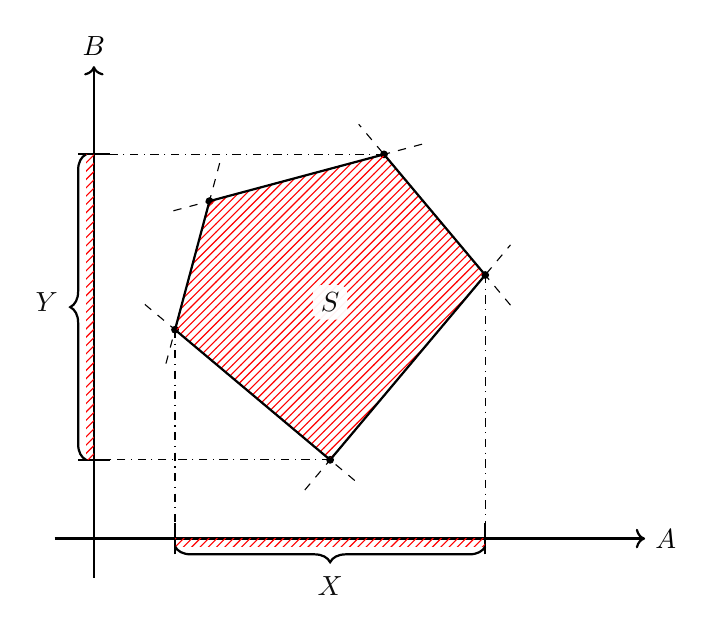
\begin{tikzpicture}[
        extend line/.style={dashed, shorten >= -0.5cm,shorten <= -0.5cm},
        set region/.style={pattern=north east lines, pattern color=red},
        set label/.style={rounded corners=1mm, inner sep=1mm, fill=white, fill opacity=0.95}
    ]
    \coordinate (ori) at (-3,-3);
    \coordinate (A) at ($(ori)+(+7,0)$);
    \coordinate (B) at ($(ori)+(0,+6)$);
    \draw[thick, ->, shorten <= -0.5cm] (ori) -- (A) node[right]{$A$};
    \draw[thick, ->, shorten <= -0.5cm] (ori) -- (B) node[above]{$B$};

    \coordinate (x1) at ( -90:2);
    \coordinate (x2) at ( +10:2);
    \coordinate (x3) at ( +70:2);
    \coordinate (x4) at (+140:2);
    \coordinate (x5) at (+190:2);
    \foreach \p in {x1,x2,x3,x4,x5} {
        \node at (\p)[circle,fill,inner sep=1pt]{}; 
        \coordinate (\p A) at ($(ori)!(\p)!(A)$);
        \coordinate (\p B) at ($(ori)!(\p)!(B)$);
    }
    \draw [thick, set region] (x1) -- (x2) -- (x3) -- (x4) -- (x5) -- cycle;
    \foreach \p/\q in {x1/x2,x2/x3,x3/x4,x4/x5,x5/x1} {
        \draw [extend line] (\p) -- (\q);
    }
    
    \foreach \p in {x2,x5} {
        \draw [dash dot] (\p) -- (\p A);
        \draw [thick] ([yshift=-2mm]\p A) -- ([yshift=+2mm]\p A);
    }
    \path[set region] (x5A) rectangle ([yshift=-1mm]x2A);

    \foreach \p in {x1,x3} {
        \draw [dash dot] (\p) -- (\p B);
        \draw [thick] ([xshift=-2mm]\p B) -- ([xshift=+2mm]\p B);
    }
    \path[set region] (x3B) rectangle ([xshift=-1mm]x1B);
    \node[set label] at (0,0) {$S$};
    \node[set label] at ([yshift=-6mm]$(ori)!(0,0)!(A)$) {$X$};
    \node[set label] at ([xshift=-6mm]$(ori)!(0,0)!(B)$) {$Y$};

    \draw[thick,decorate,decoration={brace,amplitude=2mm}] ([yshift=-1mm]x2A) -- ([yshift=-1mm]x5A);
    \draw[thick,decorate,decoration={brace,amplitude=2mm}] ([xshift=-1mm]x1B) -- ([xshift=-1mm]x3B);
\end{tikzpicture}
\end{center}

\subsection{Subset Projection}
A prototypical example wherein an adjoint triple 
\[ f_{!}, \exists_{f} \dashv f^{\ast}, f^{-1} \dashv f^{!}, \forall_{f} \]
arises is that of functions $f : X \to Y$ between sets $X$ and $Y$. The inverse image functor $f^{\ast} : \mathscr{P}Y \to \mathscr{P}X$ is defined on a subset $T \subseteq Y$
\[ f^{\ast} ( T ) = \{ x \in X : f(x) \in T \}, \]
and is functorial in the sense that if $T \subseteq T' \subseteq Y$ then $f^{\ast}(T) \subseteq f^{\ast}(T') \subseteq f^{\ast}(T)$. The adjoint functors $\exists_{f}, \forall_{f} : \mathscr{P}X \to \mathscr{P}Y$ are defined on $S \subseteq X$ as
\begin{align*}
    \exists_{f} (S) &= \{ y \in Y : \exists x \in f^{\ast}(y) : x \in S \} \\
    \forall_{f} (S) &= \{ y \in Y : \forall x \in f^{\ast}(y) : x \in S \}
\end{align*}
form an adjoint triple in the sense that $\exists_{f} \dashv f^{\ast} \dashv \forall_{f}$:
\begin{align*}
    \exists_{f} \dashv f^{\ast} : \quad \exists_{f} (S) \subseteq T &\iff S \subseteq f^{\ast}(T) \\
    f^{\ast} \dashv \forall_{f} : \quad f^{\ast}(T) \subseteq R &\iff T \subseteq \forall_{f}(R)
\end{align*}

\begin{center}
    \begin{table}
        \begin{tabular}{|c|c|c|c|c|c|c|}
            \hline
            Context & Fibration & Total $\catE$ & Base $\catE$ & Fibers & Covariant Functor & Contravariant Functor \\
            \hline
            \hline
            Subset Projection & & & & & & \\
            \hline
            Linear Quantifier Elimination & & & & & & \\
            \hline
            Non-linear Quantifier Elimination & & & & & & \\
            \hline
            Real-valued Optimization & & & & & & \\
            \hline
            General Lattice Optimization & & & & & & \\
            \hline
            Convex Projection & & & & & & \\
            \hline
            Convex Optimization & & & & & & \\
            \hline
            Resolution & & & & & & \\
            \hline
            $\ldots$ and more & & & & & & \\
            \hline
        \end{tabular}
    \end{table}
\end{center}

\subsection{Subset Projection}

\begin{center}
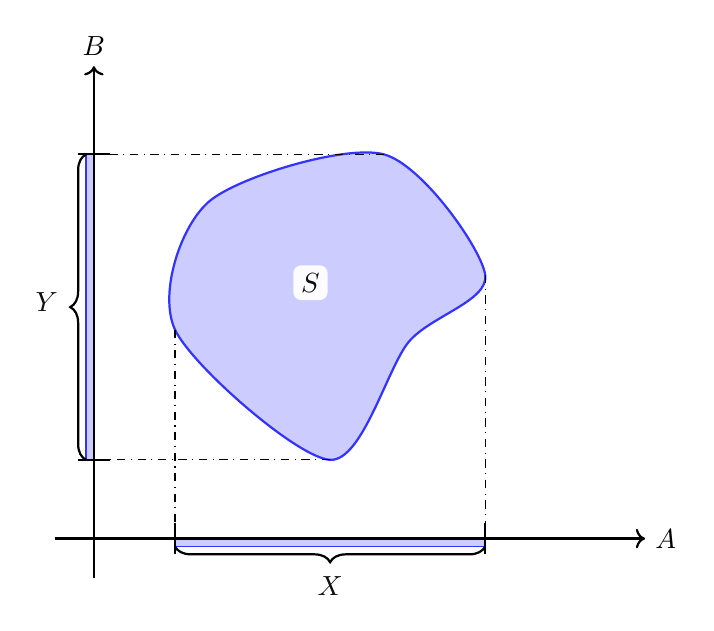
\begin{tikzpicture}[
        set region/.style={draw=blue!80, fill=blue!20},
        set label/.style={rounded corners=1mm, inner sep=1mm, fill=white, fill opacity=0.95}
    ]
    \coordinate (ori) at (-3,-3);
    \coordinate (A) at ($(ori)+(+7,0)$);
    \coordinate (B) at ($(ori)+(0,+6)$);

    \coordinate (x1) at ( -90:2);
    \coordinate (x2) at ( +10:2);
    \coordinate (x3) at ( +70:2);
    \coordinate (x4) at (+140:2);
    \coordinate (x5) at (+190:2);
    \foreach \p in {x1,x2,x3,x4,x5} {
        \coordinate (\p A) at ($(ori)!(\p)!(A)$);
        \coordinate (\p B) at ($(ori)!(\p)!(B)$);
    }
    \draw [thick, set region] plot [smooth cycle] coordinates {(x1) (+1,-0.5) (x2) (x3) (x4) (x5)};
    
    \path[set region] (x5A) rectangle ([yshift=-1mm]x2A);
    \path[set region] (x3B) rectangle ([xshift=-1mm]x1B);

    \foreach \p in {x2,x5} {
        \draw [dash dot] (\p) -- (\p A);
        \draw [thick] ([yshift=-2mm]\p A) -- ([yshift=+2mm]\p A);
    }

    \foreach \p in {x1,x3} {
        \draw [dash dot] (\p) -- (\p B);
        \draw [thick] ([xshift=-2mm]\p B) -- ([xshift=+2mm]\p B);
    }
    \node[set label] at (-0.25,+0.25) {$S$};

    \node[set label] at ([yshift=-6mm]$(ori)!(0,0)!(A)$) {$X$};
    \node[set label] at ([xshift=-6mm]$(ori)!(0,0)!(B)$) {$Y$};

    \draw[thick,decorate,decoration={brace,amplitude=2mm}] ([yshift=-1mm]x2A) -- ([yshift=-1mm]x5A);
    \draw[thick,decorate,decoration={brace,amplitude=2mm}] ([xshift=-1mm]x1B) -- ([xshift=-1mm]x3B);

    \draw[thick, ->, shorten <= -0.5cm] (ori) -- (A) node[right]{$A$};
    \draw[thick, ->, shorten <= -0.5cm] (ori) -- (B) node[above]{$B$};
\end{tikzpicture}
\end{center}

Consider a pair of sets $A$ and $B$ and a subset $S \subseteq A \times B$ of their cartesian product.  The projection morphisms associated with $A \times B$ are $p : A\times B \to A$ and $q : A \times B \to B$. The projection of the subset $S$ onto $A$ is then the subset $X \subseteq A$ defined by:
\[ X = \{ a \in A \mid \exists s \in S, p (s) = a \} \]

\begin{equation}
    S \subseteq p^{\ast} ( X ) \Longleftrightarrow \exists_p ( S ) \subseteq X
\end{equation}

\begin{center}
    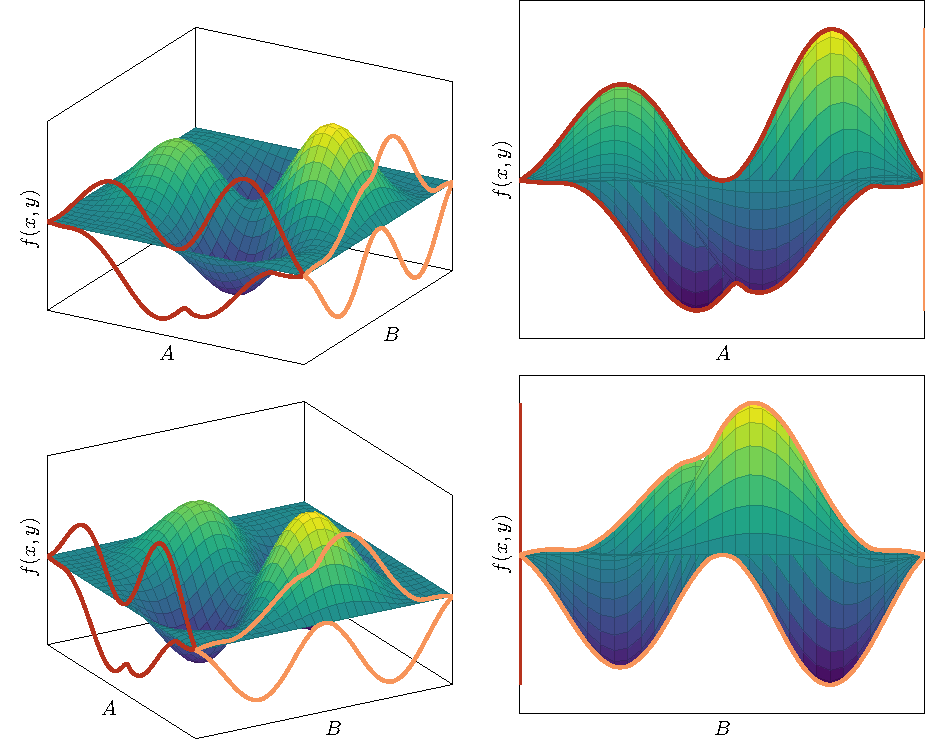
\includegraphics[]{figures/min_max_multivariate_function/figure.pdf}
\end{center}

\clearpage

\section{Categorical Notions}

The following unordered list of categorical concepts are anticipated to be utilized:
\begin{itemize}
    \item adjunctions
    \item fibered categories
    \item cleavages
    \item puesdo functors (and if cleavages are splitting, functors)
    \item Beck-Chevalley condition
    \item Frobenius reciprocity (and functors of monoidal categories)
\end{itemize}

\subsection{Cartesian Arrows}
\begin{definition}
    Let $P : \catE \to \catB$ be a functor between categories $\catE$ and $\catB$. An arrow $\phi : \alpha \to \beta$ of $\catE$ is \textit{cartesian} with respect to $P$ if for every arrow $\psi : \gamma \to \beta$ sharing a codomain with $\phi$, and for every arrow $g : P(\gamma) \to P(\alpha)$ in $\catB$ satisfying $g \circ P(\phi) = P(\psi)$, there exists a unique arrow $\theta : \gamma \to \alpha$ in $\catE$ satisfying $\phi \circ \theta = \psi$ and $P(\theta) = g$.
    \begin{equation}
        \begin{tikzcd}[row sep=small]
            \gamma \arrow[rd, dashed, "\exists!\theta"'] \arrow[rrd, bend left, "\forall\psi"] \arrow[dd, mapsto] & & \\
            & \alpha \arrow[r, "\phi"'] & \beta \arrow[dd, mapsto] \\
            P(\gamma) \arrow[rd, "\forall g"'] \arrow[rrd, bend left, "P(\psi)"' near start] & & \\
            & P(\alpha) \arrow[r, "P(\phi)"'] \arrow[from=uu, mapsto, crossing over] & P(\beta)
        \end{tikzcd}
    \end{equation}
\end{definition}

\begin{corollary}
    A cartesian morphism $\phi : \alpha \to \beta$ in $\catE$ with respect to a functor $P : \catE \to \catB$ establishes an isomorphism of categories \cite[Section~2.4.1]{lurie2009higher}\footnote{This formulation is also discussed here: \url{https://ncatlab.org/nlab/show/Cartesian+morphism\#CartInOrdCatReformulation}.}
    \begin{equation}
        \catE / \phi \cong \catE / \beta \times_{\catB / P(\beta)} \catB / P(\phi)
    \end{equation}
    where $\catE / \beta \times_{\catB / P(\beta)} \catB / P(\phi)$ is the pullback of functors.
    \begin{equation}
        \begin{tikzcd}
            \catE / \phi \ar[drr, bend left=20, "P/\phi"] \ar[ddr, bend right=40, "\mathrm{cod}"] \ar[dr, dashed, "\cong", leftrightarrow] & & \\ 
            & \catE / \beta \times_{\catB / P(\beta)} \catB / P(\phi) \ar[r] \ar[d] \ar[dr, phantom, "\ulcorner", very near start, xshift=-2em] & \catB / P(\phi) \ar[d, "\mathrm{cod}"] \\ 
            & \catE / \beta \ar[r, "P/\beta"] & \catB / P(\beta) \\ 
        \end{tikzcd}
    \end{equation}
\end{corollary} 
The pullback category $\catE / \beta \times_{\catB / P(\beta)} \catB / P(\phi)$ has morphisms associated with diagrams of $\catB$ with the following format:
\begin{equation}
    \begin{tikzcd}[row sep=large, column sep=small]
        & P(\gamma) \arrow[d, "P(\chi)"] \arrow[ddl, bend right, "f"'] \arrow[ddr, bend left, "P(\omega)"] & \\
        & P(\delta) \arrow[dl, "g"'] \arrow[dr, "P(\psi)"] & \\
        P(\alpha) \arrow[rr, "P(\phi)"] & & P(\beta)
    \end{tikzcd}
    \label{eq:pullback_category_cartesian}
\end{equation}
Evidently, if $\phi : \alpha \to \beta$ is cartesian, then there exists unique morphisms $\zeta : \gamma \to \alpha$ and $\eta : \delta \to \alpha$ such that $P(\zeta) = f$ and $P(\eta) = g$ and the following diagram of $\catE$ commutes:
\begin{equation}
    \begin{tikzcd}[row sep=large]
        & \gamma \arrow[d, "\chi"] \arrow[ddl, bend right, "\zeta"'] \arrow[ddr, bend left, "\omega"] & \\
        & \delta \arrow[dl, "\eta"'] \arrow[dr, "\psi"] & \\
        \alpha \arrow[rr, "\phi"] & & \beta
    \end{tikzcd}
    \label{eq:cartesian_over_category}
\end{equation}
Intuitively, if $\phi$ is cartesian, then in order to determine the category $\catE/\phi$ over $\phi$, it is sufficient to specify $\catE / \beta \times_{\catB / P(\beta)} \catB / P(\phi)$.

\subsection{Fibrations, Fibered Categories, and Cleavages}
\begin{definition}
    A \textit{fibered category over $\catB$} is a category $\catE$ associated to the domain of a functor, referred to as the \textit{fibration}, $P : \catE \to \catB$ with the property that for every morphism $f : a \to b$ of $\catB$ and object $\beta$ such that $P(\beta) = b$, there exists a cartesian arrow $\phi : \alpha \to \beta$ with $P(\phi) = f$.
\end{definition}
\begin{lemma}
    A fibration $P : \catE \to \catB$ is a faithful functor if and only if its fibers are thin.
\end{lemma}
\begin{proof}
    Recall that if $P : \catE \to \catB$ is a faithful functor, then by definition every pair of parallel arrows $\phi, \psi : \alpha \to \beta$ in $\catE$ satisfies 
    \begin{equation}
        \label{eq:faithfulness}
        P(\phi) = P(\psi) : P(\alpha) \to P(\beta) \implies \phi = \psi.
    \end{equation}

    $\implies$ : Assuming $P : \catE \to \catB$ is faithful functor, consider an arbitrary pair of parallel arrows $\phi, \psi : \alpha \to \beta$ in an arbitrary fiber $\catE_{x}$ over $x$; i.e. $P(\phi) = P(\psi) = \id_{x}$. In such cases, faithfulness of $P$ (Eq.~\ref{eq:faithfulness}) guarantees that $\phi = \psi$ and thus $\catE_{x}$ is a thin category.

    $\impliedby$ : If the fiber $\catE_{x}$ for every object $x$ in $\catB$ is a thin category, then clearly $P : \catE \to \catB$ \textit{must} be faithful when restricted to an individual fiber. The non-trivial case is to consider an arbitrary pair of parallel morphisms $\phi, \psi : \alpha \to \beta$ not belonging to any fibers of $\catE$. Denote $a \coloneqq P(\alpha)$ and $b \coloneqq P(\beta)$ and suppose $f \coloneqq P(\phi) = P(\psi) : a \to b$. Then, because $\catE$ is a fibered category, there exists a cartesian arrow $\zeta : \gamma \to \beta$, such that $P(\zeta) = f$ (note that $a = P(\alpha) = P(\gamma)$ but $\gamma$ is not necessarily equal to $\alpha$). Since $\zeta$ is a cartesian arrow, there exists a unique arrows $\mu, \nu: \alpha \to \gamma$ completing the top edges of the following diagram:
    \begin{equation}
        \begin{tikzcd}
            \alpha \ar[dd, mapsto] \ar[rd, "\psi"', bend right] \ar[rr,dashed,"\mu"] & & \gamma \ar[dd, mapsto] \ar[ld, "\zeta"'] & \alpha \ar[dd, mapsto] \ar[lld, "\phi", bend left=20, crossing over, near start] \ar[l, dashed, "\nu"'] \\
            & \beta  & & \\
            a \ar[rr, equals] \ar[rd, "f"', bend right] & & a \ar[r, equals] \ar[ld, "f"] & a \ar[lld,"f", bend left=20] \\
            & b \ar[from=uu, mapsto, crossing over] & & \\
        \end{tikzcd}
        .
    \end{equation}
    However, $P(\nu) = \id_{a} = P(\mu)$ and therefore $\mu$ and $\nu$ are parallel arrows in the fiber $\catE_{a}$ and therefore $\mu = \nu$ because $\catE_{a}$ is assumed thin. Therefore, $\psi = \zeta \circ \mu = \zeta \circ \nu = \phi$ and thus $P$ is a faithful functor.
\end{proof}

\begin{definition}
    A \textit{cleavage} for a fibration $P : \catE \to \catB$ is an assignment to each morphism $f : a \to b$ of $\catB$ and object $\beta$ in $\catE_b$ (i.e. $P(\beta) = b$), a unique cartesian morphism $\phi$ such that $P(\phi) = f$.
\end{definition}
\begin{equation}
    \begin{tikzcd}[column sep=large]
        f^\ast \beta_1 \ar[r, "\kappa(f ; \beta_1)"] & \beta_1 & g^\ast \ar[l, "\kappa(g ; \beta_1)"'] \beta_1 \\
        a \ar[r, "f"] \ar[u, mapsfrom] \ar[d, mapsfrom] & b \ar[u, mapsfrom] \ar[d, mapsfrom] & c \ar[l, "g"'] \ar[u, mapsfrom] \ar[d, mapsfrom] \\
        f^\ast \beta_2 \ar[r, "\kappa(f ; \beta_2)"'] & \beta_2 & g^\ast \beta_2 \ar[l, "\kappa(g ; \beta_2)"]
    \end{tikzcd}
\end{equation}
\begin{equation}
    \begin{tikzcd}[
            execute at end picture={
                \fill[blue, opacity=0.1] (-7, -0.75) rectangle (+7, -1.5) node[above left, blue!50!black, opacity=1]{$\catB$};
                \fill[red, opacity=0.1] (-8.5, +3.25) rectangle (+8.5, -0.25) node[above left, red!50!black, opacity=1]{$\catE$};
                \fill[green, opacity=0.1] (-1.75, +2.25) rectangle (+1.75, +0.25) node[above left, green!50!black, opacity=1]{$\catE_b$};
                \fill[green, opacity=0.1] (-7.75, +2.25) rectangle (-3.25, +0.25) node[above left, green!50!black, opacity=1]{$\catE_a$};
                \fill[green, opacity=0.1] (+3.25, +2.25) rectangle (+7.75, +0.25) node[above left, green!50!black, opacity=1]{$\catE_c$};
            }
        ]
        f^\ast\alpha \ar[rddd, mapsto] \ar[rr, "f^\ast\phi", dashed] \ar[rd, "f^\ast\psi", dashed] & & f^\ast\beta \ar[lddd, mapsto] \ar[rrrr, "\kappa_f(\beta)", bend left] & &
        \alpha \ar[rddd, mapsto] \ar[rr, "\phi"] \ar[rd, "\psi"] \ar[from=llll, "\kappa_f(\beta)", bend left, crossing over] \ar[from=rrrr, "\kappa_g(\beta)"', bend right, crossing over] & & \beta \ar[lddd, mapsto] \ar[from=rrrr, "\kappa_g(\beta)"', bend right, crossing over] & &
        g^\ast\alpha \ar[rddd, mapsto] \ar[rr, "g^\ast\phi", dashed] \ar[rd, "g^\ast\psi", dashed] & & g^\ast\beta \ar[lddd, mapsto] \\
        & f^\ast\gamma \ar[dd, mapsto] \ar[ru, "f^\ast\chi", dashed] \ar[rrrr, "\kappa_f(\gamma)", bend right=10, crossing over] & & & & \gamma \ar[ru, "\chi"] \ar[dd, mapsto] & & & & g^\ast\gamma \ar[dd, mapsto] \ar[ru, "g^\ast\chi", dashed] \ar[llll, "\kappa_g(\gamma)"', bend left=10, crossing over] & \\
        & & & & & & & & & & \\
        & a \ar[rrrr,"f"] & & & & b & & & & c \ar[llll, "g"'] & \\
    \end{tikzcd}
\end{equation}


\section*{Categorical Definitions}

\subsection{Hom-Functors}
For a locally small category $\catC$, the hom-functor of $\catC$ is a functor $\Hom_{\catC} : \catC^{\opcat} \times \catC \to \mathbf{Set}$ constructed in the following manner. Given objects $a,b,c,\ldots \in \catC_0$ of $\catC$, the hom-functor $\Hom_{\catC}$ maps a pair of objects $(a,b) \in (\catC^\opcat \times \catC)_0 = \catC_0 \times \catC_0 = \catC_0^2$ into the set\footnote{The collection of morphisms of type $a \to b$ forms a set because $\catC$ is locally small.} of morphisms $\catC_1$ of $\catC$ with source $a$ and target $b$. Therefore, $\Hom_{\catC}(a,b)$ is the set of morphisms in $\catC$ of type $a \to b$. Given morphisms $g^{\opcat} \in \Hom_{\catC^{\opcat}}(a,c)$ and $h \in \Hom_{\catC}(b,d)$, the hom-functor $\Hom_{\catC}$ constructs a function
\[ \Hom_{\catC}(g^{\opcat}, h) : \Hom_{\catC}(a,b) \to \Hom_{\catC}(c,d) \]
which takes a morphism $f : a \to b \in \Hom_{\catC}(a,b)$ and produces the morphism $h \circ f \circ g : c \to d \in \Hom_{\catC}(c,d)$. Graphically,
\[
    \Hom_{\catC}(g^{\opcat}, h)
    \left(
    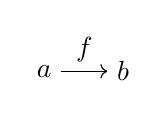
\begin{tikzpicture}
        \draw (0,0) node(a){$a$};
        \draw (1,0) node(b){$b$};
        \draw[->] (a) to node[above, midway]{$f$} (b);
    \end{tikzpicture}
    \right)
    =
    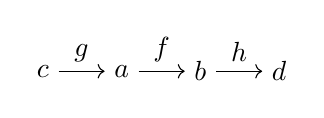
\begin{tikzpicture}
        \draw (0,0) node(c){$c$};
        \draw (1,0) node(a){$a$};
        \draw (2,0) node(b){$b$};
        \draw (3,0) node(d){$d$};
        \draw[->] (c) to node[above, midway]{$g$} (a);
        \draw[->] (a) to node[above, midway]{$f$} (b);
        \draw[->] (b) to node[above, midway]{$h$} (d);
    \end{tikzpicture}
\]

\subsection{Adjoint Functors}
Given two categories $\mathscr{C}$ and $\mathscr{D}$, a pair of functors $L : \mathscr C \to \mathscr D, R : \mathscr D \to \mathscr C$ are called an \textit{adjoint pair}, denoted $L \dashv R$ or
\[
    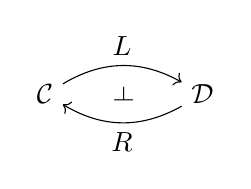
\begin{tikzpicture}
        \draw (0,0) node(c){$\catC$};
        \draw (2,0) node(d){$\catD$};
        \draw[->] (c) to[bend left] node[above, midway]{$L$} (d);
        \draw[->] (d) to[bend left] node[below, midway]{$R$} (c);
        \draw (1,0) node[rotate=-90]{$\dashv$};
    \end{tikzpicture}
\]
if there exists a natural isomorphism $\alpha$ between the following pair of hom-functors of type $\mathscr C^{\opcat} \times \mathscr D \to \mathbf{Set}$:
\[ \Hom_{\mathscr D}(L^{\opcat}(-), -) \stackrel{\alpha}{\simeq} \Hom_{\mathscr C}(-, R(-)) \]
This relationship can be depicted graphically as $2$-cell (and its inverse) in $\mathbf{Cat}$,
\[
    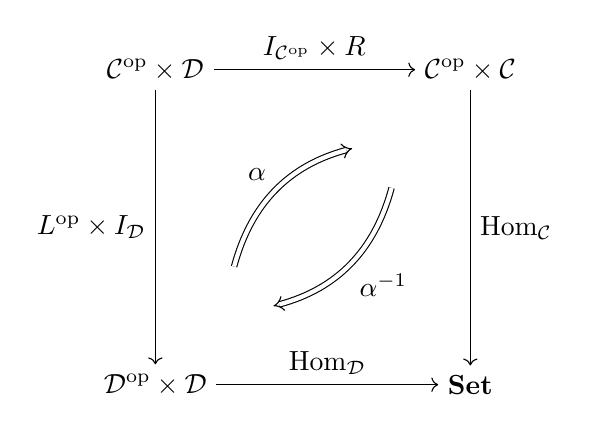
\begin{tikzpicture}
        \draw (0,4) node(tl){$\catC^\opcat \times \catD$};
        \draw (4,4) node(tr){$\catC^\opcat \times \catC$};

        \draw (0,0) node(bl){$\catD^{\opcat} \times \catD$};
        \draw (4,0) node(br){$\mathbf{Set}$};
        \draw[->] (tl) to node[midway, above]{$I_{\catC^{\opcat}} \times R$} (tr);
        \draw[->] (bl) to node[midway, above]{$\Hom_{\catD}$} (br);
        \draw[->] (tl) to node[midway, left]{$L^{\opcat} \times I_{\catD}$} (bl);
        \draw[->] (tr) to node[midway, right]{$\Hom_{\catC}$} (br);

        \draw[double equal sign distance, -implies] (1,1.5) to[bend left] node[above left]{$\alpha$} (2.5,3);
        \draw[double equal sign distance, -implies] (3,2.5) to[bend left] node[below right]{$\alpha^{-1}$} (1.5,1);
    \end{tikzpicture}
\]
Concretely, the naturality of $\alpha$ means that for every morphism $(f^{\opcat} : b \to a, g : c \to d) \in (\catC^{\opcat} \times \catD)_1$ the components $\alpha_{(b,c)}$ and $\alpha_{(a,d)}$ of $\alpha$ make the following square commute:
\[
    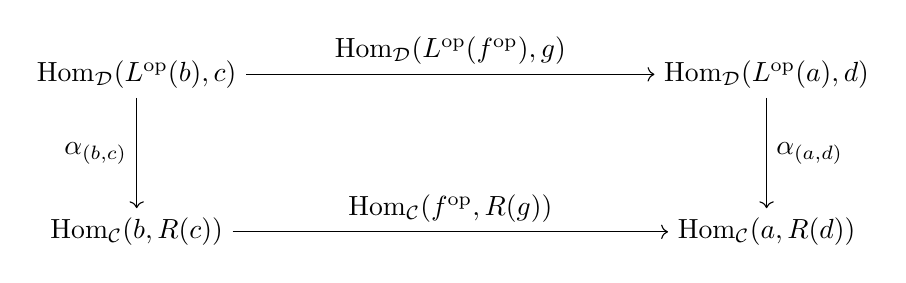
\begin{tikzpicture}
        \draw (0,2) node(tl){$\Hom_{\catD}(L^{\opcat}(b), c)$};
        \draw (8,2) node(tr){$\Hom_{\catD}(L^{\opcat}(a), d)$};
        \draw[->] (tl) to node[midway, above]{$\Hom_{\catD}(L^{\opcat}(f^{\opcat}), g)$} (tr);

        \draw (0,0) node(bl){$\Hom_{\catC}(b, R(c))$};
        \draw (8,0) node(br){$\Hom_{\catC}(a, R(d))$};
        \draw[->] (bl) to node[midway, above]{$\Hom_{\catC}(f^{\opcat}, R(g))$} (br);

        \draw[->] (tl) to node[midway, left]{$\alpha_{(b,c)}$} (bl);
        \draw[->] (tr) to node[midway, right]{$\alpha_{(a,d)}$} (br);
    \end{tikzpicture}
\]

\subsection{Beck-Chevalley Conditions}

The Beck-Chevalley Conditions are conditions that may or may not be satisfied by a quadruplet of functors $F,H,G,K$ which form a natural isomorphism $\alpha : K F \Rightarrow H G$ square:

\[
    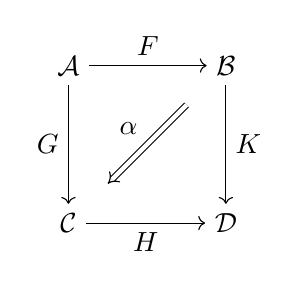
\begin{tikzpicture}
        \draw (-1,+1) node(tl){$\catA$};
        \draw (+1,+1) node(tr){$\catB$};
        \draw (-1,-1) node(bl){$\catC$};
        \draw (+1,-1) node(br){$\catD$};

        \draw[->] (tl) to node[above]{$F$} (tr);
        \draw[->] (tl) to node[left ]{$G$} (bl);
        \draw[->] (bl) to node[below]{$H$} (br);
        \draw[->] (tr) to node[right]{$K$} (br);

        \draw[double equal sign distance, -implies] (+0.5,+0.5) to node[above left]{$\alpha$} (-0.5,-0.5);
    \end{tikzpicture}
\]
To define the \textit{left} Beck-Chevalley condition, one needs functors $F_L : \catB \to \catA$ and $H_L : \catD \to \catA$ which are respectively left adjoint functors to $F$ and $H$, 

\[
    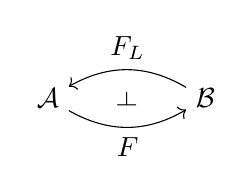
\begin{tikzpicture}
        \draw (-1,+1) node(tl){$\catA$};
        \draw (+1,+1) node(tr){$\catB$};

        \draw[->] (tl) to[bend right] node[below]{$F$} (tr);
        \draw[->] (tr) to[bend right] node[above]{$F_L$} (tl);
        \draw (0,+1) node[rotate=-90]{$\dashv$};
    \end{tikzpicture}
    ,
    \qquad 
    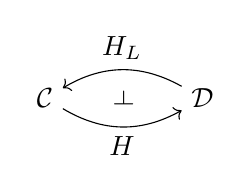
\begin{tikzpicture}
        \draw (-1,-1) node(bl){$\catC$};
        \draw (+1,-1) node(br){$\catD$};

        \draw[->] (bl) to[bend right] node[below]{$H$} (br);
        \draw[->] (br) to[bend right] node[above]{$H_L$} (bl);
        \draw (0,-1) node[rotate=-90]{$\dashv$};
    \end{tikzpicture}
    .
\]
Using these left adjoint functors, it becomes possible to construct a natural transformation $\beta : KH_L \Rightarrow GF_L$ from $\alpha$\footnote{The natural transformations $\alpha$ and $\beta$ are known as \textit{mates} or \textit{conjugates}.}. Graphically, $\beta$ can be identified as the outer cell of the following diagram:
\[
    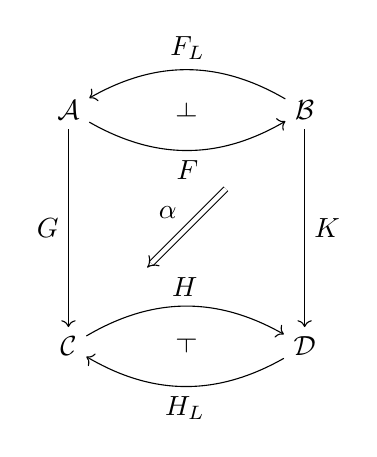
\begin{tikzpicture}
        \draw (-1.5,+1.5) node(tl){$\catA$};
        \draw (+1.5,+1.5) node(tr){$\catB$};
        \draw (-1.5,-1.5) node(bl){$\catC$};
        \draw (+1.5,-1.5) node(br){$\catD$};

        \draw[->] (tl) to[bend right] node[below]{$F$} (tr);
        \draw[->] (tr) to[bend right] node[above]{$F_L$} (tl);
        \draw (0,+1.5) node[rotate=-90]{$\dashv$};
        \draw[->] (tl) to node[left ]{$G$} (bl);
        \draw[->] (bl) to[bend left ] node[above]{$H$} (br);
        \draw[->] (br) to[bend left ] node[below]{$H_L$} (bl);
        \draw (0,-1.5) node[rotate=+90]{$\dashv$};
        \draw[->] (tr) to node[right]{$K$} (br);

        \draw[double equal sign distance, -implies] (+0.5,+0.5) to node[above left]{$\alpha$} (-0.5,-0.5);
    \end{tikzpicture},
    \qquad
    \text{i.e.}
    \qquad
    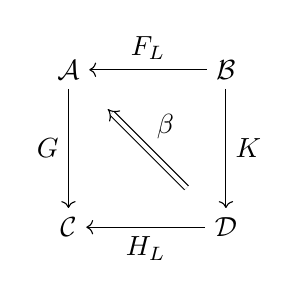
\begin{tikzpicture}
        \draw (-1,+1) node(tl){$\catA$};
        \draw (+1,+1) node(tr){$\catB$};
        \draw (-1,-1) node(bl){$\catC$};
        \draw (+1,-1) node(br){$\catD$};

        \draw[->] (tr) to node[above]{$F_L$} (tl);
        \draw[->] (tl) to node[left ]{$G$} (bl);
        \draw[->] (br) to node[below]{$H_L$} (bl);
        \draw[->] (tr) to node[right]{$K$} (br);

        \draw[double equal sign distance, -implies] (+0.5,-0.5) to node[above right]{$\beta$} (-0.5,+0.5);
    \end{tikzpicture}.
\]
Although the natural transformation $\alpha$ is assumed to be a natural isomorphism, the natural transformation $\beta$ need not be; if $\beta$ happens to be a natural isomorphism, then we say that the original square satisfies the \textit{left} Beck-Chevalley condition\footnote{Are the left adjoints $F_L, H_L$ unique? If not, it might be better to say the original square satifies the left Beck-Chevalley condition with respect to $F_L, H_L$.}. The \textit{right} Beck-Chevalley condition is defined analogously with functors $F_R, H_R$ which are respectively right adjoints $F \dashv F_R$ and $H \dashv H_R$.

\subsection{The Equivalence of Puesdofunctors and Fibrations}

Given a functor $P : \catE \to \catB$ which is also a Grothendieck fibration equipped with a cleavage (i.e. a choice of cartesian morphism $\phi \in \Hom_{\catE}(e', e)$ for each $f \in \Hom_{\catB}(a,P(e))$ such that $P(\phi) = f$), it is possible to construct a pseudofunctor (read weak $2$-functor between weak $2$-categories) $\pi : \catB^{\opcat} \to \mathbf{Cat}$. In particular, each object $b \in \catB_0$ is mapped to the \textit{sub-category} $\pi(b) = \catE_b$ of $\catE$ whose objects are those which map to $b$ under $P$ and whose morphism are those which map to $\id_{b}$ under $P$; $\catE_b$ is the fibre category over $b$ with respect to $P$. For each morphism $f \in \Hom_{\catB}(a,b)$ in $\catB$, the pseudofunctor $\pi$ maps $f^{\opcat} : b \to a$ onto a functor $\pi(f^{\opcat}) = f^{\ast} : \catE_{b} \to \catE_{a}$ which is defined accordingly:
\[
    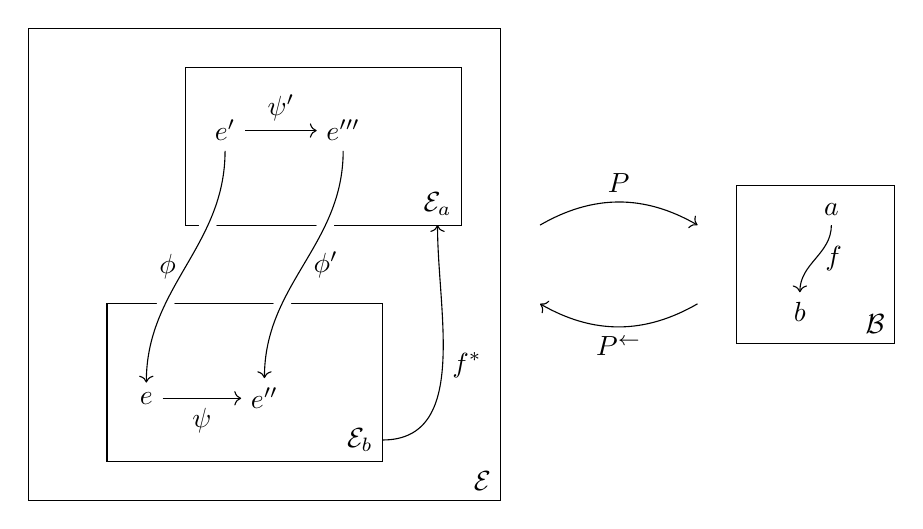
\begin{tikzpicture}
        \begin{scope}[shift={(-4.5,0)}]
            \draw (-3,+3) rectangle (+3,-3) node[above left]{$\catE$};
            \begin{scope}[shift={(-1,+2.5)}]
                \draw (0,0) rectangle (+3.5,-2) node[above left](catEa){$\catE_a$};
                \draw (+0.5, -0.8) node(e2){$e'$};
                \draw (+2, -0.8) node(e4){$e'''$};
                \draw[->] (e2) to node[above]{$\psi'$} (e4);
            \end{scope}
            \begin{scope}[shift={(-2,-0.5)}]
                \draw (0,0) rectangle (+3.5,-2) node[above left](catEb){$\catE_b$};
                \draw (+0.5, -1.2) node(e1){$e$};
                \draw (+2, -1.2) node(e3){$e''$};
                \draw[->] (e1) to node[below]{$\psi$} (e3);
            \end{scope}
            \draw[white, line width=2mm] (e2) to[out=-90,in=+90] (e1);
            \draw[white, line width=2mm] (e4) to[out=-90,in=+90] (e3);
            \draw[->] (e2) to[out=-90,in=+90] node[left ]{$\phi$} (e1);
            \draw[->] (e4) to[out=-90,in=+90] node[right]{$\phi'$} (e3);
            \draw[->] (catEb) to[out=0,in=-90] node[right]{$f^{\ast}$} (catEa);
        \end{scope}
        \begin{scope}[shift={(+1.5,+1)}]
            \draw (0,0) rectangle (+2,-2) node[above left]{$\catB$};
            \draw (+1.2, -0.3) node(a){$a$};
            \draw (+0.8,-1.6) node(b){$b$};
            \draw[->] (a) to[out=-90,in=+90] node[right]{$f$} (b);
        \end{scope}
        \draw[->] (-1,+0.5) to[bend left ] node[above]{$P$} (+1, 0.5);
        \draw[<-] (-1,-0.5) to[bend right] node[below]{$P^{\leftarrow}$} (+1, -0.5);
    \end{tikzpicture}
\]
Given an object $e \in (\catE_b)_0$, the functor $f^{\ast}$ finds the unique cartesian morphism $\phi \in \Hom_{\catE}(e',e)$ as specified by the cleavage and assigns $f^{\ast}(e) = e'$. Next, given a morphism $\psi \in \Hom_{\catE_{b}}(e, e'')$, the functor $f^{\ast}$ first finds the unique cartesian morphisms $\phi \in \Hom_{\catE}(e', e)$ and $\phi' \in \Hom_{\catE}(e''', e'')$. Then, because $g = \id_a$ completes the following diagram
\[
    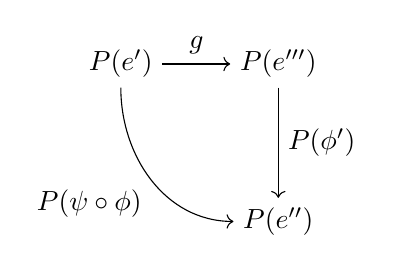
\begin{tikzpicture}
        \draw (-1,+1) node(tl){$P(e')$};
        \draw (+1,+1) node(tr){$P(e''')$};
        \draw (+1,-1) node(br){$P(e'')$};

        \draw[->] (tl) to node[above]{$g$} (tr);
        \draw[->] (tl) to[out=-90, in=180] node[below left]{$P(\psi\circ\phi)$} (br);
        \draw[->] (tr) to node[right]{$P(\phi')$} (br);
    \end{tikzpicture}
    \quad=\quad
    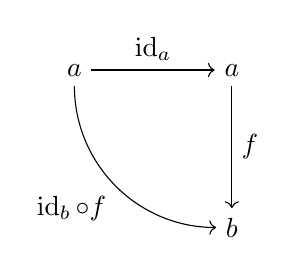
\begin{tikzpicture}
        \draw (-1,+1) node(tl){$a$};
        \draw (+1,+1) node(tr){$a$};
        \draw (+1,-1) node(br){$b$};

        \draw[->] (tl) to node[above]{$\id_{a}$} (tr);
        \draw[->] (tl) to[out=-90, in=180] node[below left]{$\id_{b} \circ f$} (br);
        \draw[->] (tr) to node[right]{$f$} (br);
    \end{tikzpicture},
\]
and because $\phi'$ is cartesian, there must exist a unique $\psi' \in \Hom_{\catE_a}(e', e''')$ such that $\psi \circ \phi = \phi' \circ \psi'$. For each $\psi \in \Hom_{\catE_b}(e, e'')$, the functor $f^{\ast}$ selects this unique morphism $f^{\ast}(\psi) = \psi'$. In summary, the pseudofunctor $\pi : \catB^{\opcat} \to \mathbf{Cat}$ induced by $P : \catE \to \catB$ is defined on objects $b \in \catB_{0}$ as $\pi(b) = \catE_{b}$ and on morphisms $f \in \catB_{1}$ as $\pi(f) = f^{\ast}$ and forms a functor \textcolor{red!50!black}{[TODO: figure out the `pseudo' part of the pseudofunctorality.]}.

\subsection{Slice and Coslice Categories}

Given a category $\catC$ and an object $c \in \catC_0$ of $\catC$, the \textit{slice category} (or \textit{over category}) $\catC/c$ is the ``stuff in $\catC$ that is on top of $c$''. Specifically, the objects of $\catC/c$ are all the morphisms $f \in \catC_1$ from $\catC$ whose codomain is $\cod(f) = c$ (alternatively you could write $(\catC/c)_0 = \Hom_{\catC}(-,c)$). A morphism of $\catC/c$ between objects $f : a \to c, g : b \to c \in (\catC/c)_0$ is a commuting triangle completed by a third morphism $h : a \to b \in \catC_1$:

\[
    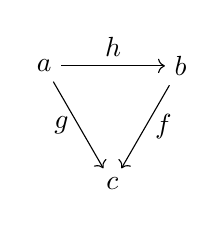
\begin{tikzpicture}
        \draw (150:1) node(tl){$a$};
        \draw ( 30:1) node(tr){$b$};
        \draw (270:1)node(bm){$c$};

        \draw[->] (tl) to node[below,left ]{$g$} (bm);
        \draw[->] (tr) to node[below,right]{$f$} (bm);

        \draw[->] (tl) to node[above]{$h$} (tr);
    \end{tikzpicture}
\]
Composition of morphisms in $\catC/c$ is induced by the composition of morphisms in $\catC$:
\[
    \left(
    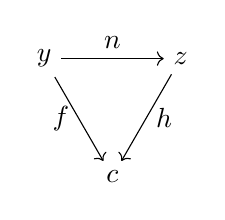
\begin{tikzpicture}
        \draw (150:1) node(tl){$y$};
        \draw ( 30:1) node(tr){$z$};
        \draw (270:1) node(bm){$c$};

        \draw[->] (tl) to node[below,left ]{$f$} (bm);
        \draw[->] (tr) to node[below,right]{$h$} (bm);

        \draw[->] (tl) to node[above]{$n$} (tr);
    \end{tikzpicture}
    \right)
    \circ_{\catC/c}
    \left(
    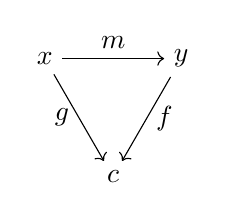
\begin{tikzpicture}
        \draw (150:1) node(tl){$x$};
        \draw ( 30:1) node(tr){$y$};
        \draw (270:1) node(bm){$c$};

        \draw[->] (tl) to node[below,left ]{$g$} (bm);
        \draw[->] (tr) to node[below,right]{$f$} (bm);

        \draw[->] (tl) to node[above]{$m$} (tr);
    \end{tikzpicture}
    \right)
    =
    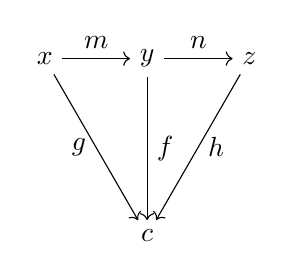
\begin{tikzpicture}
        \draw (150:1.5) node(tl){$x$};
        \draw ( 90:0.75) node(tm){$y$};
        \draw ( 30:1.5) node(tr){$z$};
        \draw (270:1.5) node(bm){$c$};

        \draw[->] (tl) to node[below,left ]{$g$} (bm);
        \draw[->] (tm) to node[right]{$f$} (bm);
        \draw[->] (tr) to node[below,right]{$h$} (bm);

        \draw[->] (tl) to node[above]{$m$} (tm);
        \draw[->] (tm) to node[above]{$n$} (tr);
    \end{tikzpicture}
\]

The assignment of an overcategory $\catC/c$ to each object $c$ can be extended to a \textit{slice functor} $\catC / (-) : \catC \to \mathbf{Cat}$ in the following sense. For objects $c \in \catC_0$, the slice functor takes $c$ to the slice category $\catC/c$; for morphisms $f : a \to b \in \catC_1$, the slice functor takes $f$ to the functor $\catC / f : \catC / a \to \catC / b$ defined graphically; for every morphism of $\catC / a$ (commuting triangle in $\catC$ over $a$), contruct the morphism of $\catC / b$ (commuting triangle in $\catC$ over $b$) as follows:
\[
    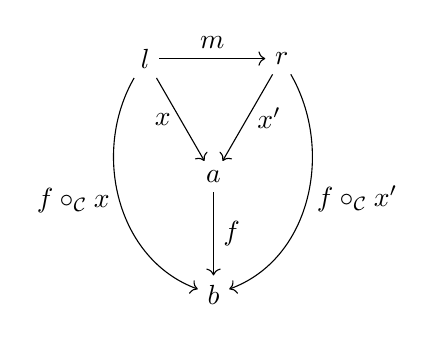
\begin{tikzpicture}
            \draw (150:1) node(tl){$l$};
            \draw ( 30:1) node(tr){$r$};
            \draw (270:1) node(bm){$a$};
            \draw (270:2.5) node(bb){$b$};

            \draw[->] (tl) to node[below,left ]{$x$}  (bm);
            \draw[->] (tr) to node[below,right]{$x'$} (bm);
            \draw[->] (tl) to[out=-120, in=+160] node[below,left ]{$f \circ_{\catC} x$}  (bb);
            \draw[->] (tr) to[out= -60, in= +20] node[below,right]{$f \circ_{\catC} x'$} (bb);
            \draw[->] (tl) to node[above]{$m$} (tr);
            \draw[->] (bm) to node[right]{$f$} (bb);
    \end{tikzpicture}
\]
where the inner triangle is a morphism of $\catC/a$ and the outer triangle is a morphism of $\catC/b$ given by the functor $\catC/f$.

Given a category $\catC$ and an object $c \in \catC_0$ of $\catC$ the \textit{coslice category} (or \textit{under category}) $c/\catC$ is the ``stuff in $\catC$ that is underneath $c$''. Specifically, the objects of $c/\catC$ are all the morphisms $f \in \catC_1$ from $\catC$ whose domain is $\dom(f) = c$ (alternatively you could write $(c/\catC)_0 = \Hom_{\catC}(c,-)$). A morphism of $c/\catC$ between objects $f : c \to a, g : c \to b \in (c/\catC)_0$ is a commuting triangle completed by a third morphism $h : a \to b \in \catC_1$:

\[
    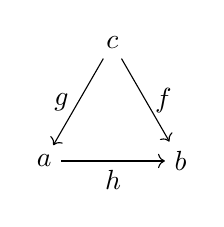
\begin{tikzpicture}
        \draw (210:1) node(tl){$a$};
        \draw (330:1) node(tr){$b$};
        \draw ( 90:1) node(bm){$c$};

        \draw[<-] (tl) to node[below,left ]{$g$} (bm);
        \draw[<-] (tr) to node[below,right]{$f$} (bm);
        \draw[->] (tl) to node[below]{$h$} (tr);
    \end{tikzpicture}
\]
Everything about coslice categories is defined as expected analogously to that of a slice categories.
\textcolor{red!50!black}{[TODO: determine how the details of the Grothendieck construction transform the slice (pseudo-)functor $\catC / (-) : \catC \to \mathbf{Cat}$ into the codomain fibration.]}
\subsection{The Pullback and Pushforward Functors}

Given a category $\catC$ and a morphism $f : a \to b \in \catC_1$, the image of $f$ under the slice functor $\catC / (-)$ produces a functor $\catC / f : \catC / a \to \catC / b$ between slice categories of $\catC$ in the ``same direction'' as $f$ \textcolor{red!50!black}{TODO: confirm that $\catC / f$ is the pushforward functor $f_{!}$ of $f \in \catC_1$.}

If the given category $\catC$ admits pullbacks, in becomes possible to define, for a morphism $f : a \to b$ a pullback functor $f^{*} : \catC / b \to \catC / a$. Given a morphism in $\catC/b$ (commuting triangle in $\catC$ with base at $b$),
\[
    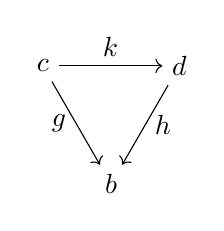
\begin{tikzpicture}
        \begin{scope}[shift={(+3,0)}]
            \draw (150:1) node(ltl){$c$};
            \draw ( 30:1) node(ltr){$d$};
            \draw (270:1) node(lbm){$b$};

            \draw[->] (ltl) to node[below,left ]{$g$}  (lbm);
            \draw[->] (ltr) to node[below,right]{$h$} (lbm);
            \draw[->] (ltl) to node[above]{$k$} (ltr);
        \end{scope}
    \end{tikzpicture}
\]
the pullback functor $f^{\ast} : \catC / b \to \catC / a$ associated with $f$ takes the objects $g : c \to b, h : d \to b$ of $\catC/b$ (morphisms in $\catC$) completes the pullback squares associated with $f$
\[
    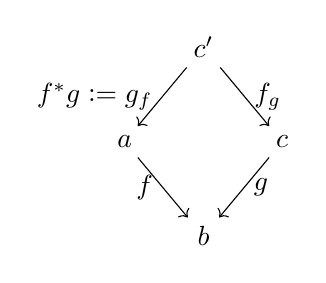
\begin{tikzpicture}
        \begin{scope}[shift={(0,0)}]
            \draw ( 90:1.2) node(t){$c'$};
            \draw (180:1) node(l){$a$};
            \draw (  0:1) node(r){$c$};
            \draw (270:1.2) node(b){$b$};

            \draw[->] (l) to node[below,left ]{$f$} (b);
            \draw[->] (r) to node[below,right]{$g$} (b);
            \draw[->] (t) to node[above,left ]{$f^{\ast}g \vcentcolon= g_{f}$} (l);
            \draw[->] (t) to node[above,right]{$f_{g}$} (r);
        \end{scope}
    \end{tikzpicture}
    \qquad
    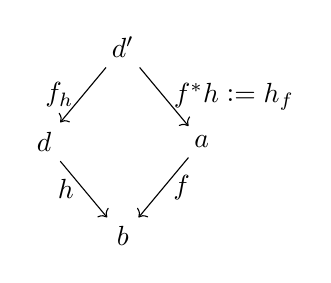
\begin{tikzpicture}
        \begin{scope}[shift={(0,0)}]
            \draw ( 90:1.2) node(t){$d'$};
            \draw (180:1) node(l){$d$};
            \draw (  0:1) node(r){$a$};
            \draw (270:1.2) node(b){$b$};

            \draw[->] (l) to node[below,left ]{$h$} (b);
            \draw[->] (r) to node[below,right]{$f$} (b);
            \draw[->] (t) to node[above,left ]{$f_{h}$} (l);
            \draw[->] (t) to node[above,right]{$f^{\ast}h \vcentcolon= h_{f}$} (r);
        \end{scope}
    \end{tikzpicture}
\]
where a subscript notation $g_{f}$ means ``the pullback of $g$ along $f$''. Defining the action of $f^{\ast} : \catC / b \to \catC / a$ on objects to be $f^{\ast}g = g_{f}$ and $f^{\ast}h = h_{f}$, the action on morphisms in $\catC / b$ is defined by composing the pullback squares with the commuting triangle morphism:
\[
    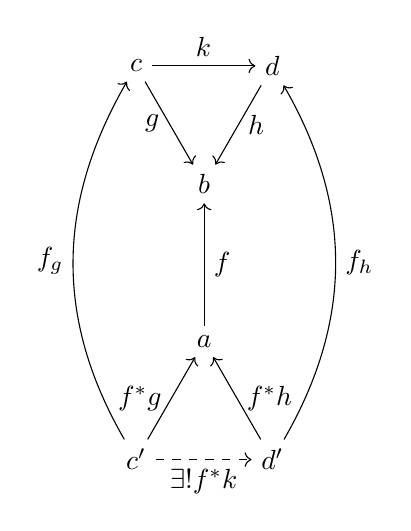
\begin{tikzpicture}
        \begin{scope}[shift={(0,+2)}]
            \draw (150:1) node(t1){$c$};
            \draw ( 30:1) node(t2){$d$};
            \draw (270:1) node(t3){$b$};

            \draw[->] (t1) to node[below,left ]{$g$}  (t3);
            \draw[->] (t2) to node[below,right]{$h$} (t3);
            \draw[->] (t1) to node[above]{$k$} (t2);
        \end{scope}

        \begin{scope}[shift={(0,-2)}]
            \draw (210:1) node(b1){$c'$};
            \draw (330:1) node(b2){$d'$};
            \draw ( 90:1) node(b3){$a$};

            \draw[->] (b1) to node[below,left ]{$f^{\ast}g$} (b3);
            \draw[->] (b2) to node[below,right]{$f^{\ast}h$} (b3);
            \draw[dashed, ->] (b1) to node[below]{$\exists! f^{\ast}k$} (b2);
        \end{scope}
        \draw[->] (b1) to[out=+120, in=-120] node[left ]{$f_{g}$} (t1);
        \draw[->] (b2) to[out=+ 60, in=- 60] node[right]{$f_{h}$} (t2);
        \draw[->] (b3) to node[right]{$f$} (t3);
    \end{tikzpicture}
\]
The commuting triangle in $\catC / a$ appearing at the bottom is completed by a unique morphism \textcolor{red!50!black}{[TODO: why does this morphism need to be unique and exist?]} denoted to be $f^{\ast}k$ ($\neq k_{f}$ obviously). The functoriality of $f^{\ast}$ has a simple proof found here \url{https://proofwiki.org/wiki/Pullback_Functor_is_Functor}.

\subsection{Functors of Monoidal Categories}

\textcolor{red!50!black}{[TODO]}

\subsection{Frobenius Reciprocity}

\textcolor{red!50!black}{[TODO]}

\section*{Comments on selected references}
This section is temporary and reserved for recording comments toward various references.
\begin{itemize}
    \item \citeauthor{vistoli2004notes}~\cite{vistoli2004notes}
    \item \citeauthor{street1974fibrations}~\cite{street1974fibrations}
    \item \citeauthor{koudenburg2018categorical}~\cite{koudenburg2018categorical}
    \item \citeauthor{brown2009algebraic}~\cite{brown2009algebraic}
    \item \citeauthor{lurie2009higher}~\cite{lurie2009higher}
    \item \citeauthor{shulman2008framed}~\cite{shulman2008framed}
\end{itemize}

\printbibliography
\end{document}
